\documentclass[11pt,twoside]{report}
\usepackage[table,xcdraw]{xcolor}
\usepackage[utf8]{inputenc}
\usepackage{graphicx}
\usepackage{wrapfig}
\usepackage[a4paper, width=150mm, top=25mm, bottom=30mm, bindingoffset=20mm]{geometry}
\usepackage[titletoc, title,header]{appendix}
\usepackage{pdfpages}
\usepackage{natbib}
\usepackage{dirtytalk}
\usepackage{pdflscape}
\usepackage{longtable}
%\usepackage{showframe}
\usepackage{multirow}
\usepackage{textcomp}
\usepackage{fancyhdr}
\usepackage{tikz}
\usepackage{setspace}
\usepackage{helvet}
\usepackage{hyphenat}
\usepackage[hidelinks]{hyperref}
%\usepackage[autostyle]{csquotes}
\usepackage{soul}
\usepackage{tikz}
\usepackage{rotating}
\usepackage{caption}
\usetikzlibrary{calc}
\usepackage[export]{adjustbox}
\usepackage{amsmath}
\usepackage{glossaries}
\usepackage{tabularx}
\makenoidxglossaries
\newglossaryentry{APWG}{
    name={APWG},
    description={Anti Phishing Working Group}
}

\newglossaryentry{TLS}{
    name={TLS},
    description={Transport Layer Security}
}
\newglossaryentry{HTTPS}{
    name={HTTPS},
    description={Hypertext Transfer Protocol Secure}
}

\newglossaryentry{HTTP}{
    name={HTTP},
    description={Hypertext Transfer Protocol}
}

\newglossaryentry{API}{
    name={API},
    description={Application Programming Interface}
}

\newglossaryentry{GSB}{
    name={GSB},
    description={Google Safe Browsing}
}

\newglossaryentry{SSL}{
    name={SSL},
    description={Secure Socket Layer}
}
\renewcommand{\familydefault}{\sfdefault}
\def\checkmark{\tikz\fill[scale=0.4](0,.35) -- (.25,0) -- (1,.7) -- (.25,.15) -- cycle;} 
\pagestyle{fancy}
\fancyhf{}
\fancyhead[LE, RO]{\thepage}
\fancyhead[LO, RE]{\leftmark}
\fancyfoot[c]{Bournemouth University, Department of Computing and Informatics, Final Year Project}
\setlength{\headheight}{13.6pt}
% Recommended linespread is 1.5
\linespread{1.5}
%\bibliographystyle{buHarvard}
\bibpunct{(}{)}{,}{a}{}{ }
\usepackage{packages/multibib}
\newcites{r}{References}
\newcites{b}{Bibliography}
\graphicspath{ {figures/}{appendices/} }
\footskip = 15mm

\usepackage{emptypage}

\usepackage{titlesec}
\titleformat{\chapter}[hang]
	{\normalfont\Huge\bfseries}{\thechapter\quad}{0pt}{\Huge}
\titlespacing*{\chapter}{0pt}{0pt}{20pt}


\begin{document}

%!TEX root = ../../main.tex

\begin{titlepage}
    \centering
\begin{tikzpicture}[overlay,remember picture]
    \draw [line width=1mm]
        ($ (current page.north west) + (2cm,-2cm) $)
        rectangle
        ($ (current page.south east) + (-2cm,2cm) $);
\end{tikzpicture}

\vspace*{1em}\hspace*{-1cm}
\includegraphics[width=3.5cm, left]{figures/unilogo.png}

\begin{center}
\huge{FACULTY OF SCIENCE \& TECHNOLOGY}
\\
\normalsize\vspace{6em}

\LARGE{
BSc (Hons) Forensic Computing \& Security
}
\\*
\LARGE{
May 2020
}

\normalsize\vspace{6em}

\LARGE{
URL based multi-layered anti-phishing 

detection system
}
\\*
\normalsize\vspace{4em}
\LARGE{by}
\\*
\normalsize\vspace{4em}
\LARGE{
Andrei Butnaru
}

\end{center}
\end{titlepage}
\cleardoublepage





\pagenumbering{Roman}

%!TEX root = ../../main.tex

\vspace*{\fill}
\begingroup
\centering
Faculty of Science \& Technology

Department of Computing and Informatics

Final Year Project

\endgroup
\vspace*{\fill}

\cleardoublepage


%!TEX root = ../main.tex
\chapter*{Abstract}

The history of the past 30 years shows that cyber-attacks are here to stay, and the security industry offers a great deal of protection, but threats come in many shapes and forms. Virtually all the threats reside in the software-hardware area but one. This threat is the manipulation of people to act as a proxy for the threat actor and carry out malicious actions, process called phishing.

Phishing has made a name for itself across the years. By taking advantage of human nature or flaws, the malicious actor is able to bypass most of, if not all security protections. The ease of conducting such an attack compared to other has popularised the belief that "humans are the weakest link in the cyber-security chain". The work presented in this dissertation will explore a method to mitigate some of the responsability from the target of phishing. Furthermore it aims to do that while being lightweight and performant, but most importantly actionable with minimal technical literacy.
%[The text within the square brackets must be deleted along with the square brackets when finalising your own abstract. 

%The abstract for an undergraduate dissertation should be between 200 - 350 words.

%Arial, Normal, 11pt with 1.2 or 1.5 line spacing should be used. The text in this part has 1.5 line spacing.

%An abstract is a brief, accurate and comprehensive summary of the entire dissertation. It is the first thing to be read by your examiners to help them know the brief content of the dissertation. It also serves as a “sales pitch” to form the first impression of your work. 

%A good abstract should be accurate, self-contained, concise, specific and clear. A quick way to assess the quality of your abstract is to check whether it answers the questions why, how, what and so what.

%It is easier to write the Abstract the last.]

%!TEX root = ../main.tex
\chapter*{Dissertation Declaration}
{\linespread{1.0} %The BU template dictates this to be this line spacing
	I agree that, should the University wish to retain it for reference purposes, a copy of my dissertation may be held by Bournemouth University normally for a period of 3 academic years. I understand that once the retention period has expired my dissertation will be destroyed.

	\section*{Confidentiality}
	I confirm that this dissertation does not contain information of a commercial or confidential nature or include personal information other than that which would normally be in the public domain unless the relevant permissions have been obtained. In particular any information which identifies a particular individual's religious or political beliefs, information relating to their health, ethnicity, criminal history or sex life has been anonymised unless permission has been granted for its publication from the person to whom it relates.

	\section*{Copyright}
	The copyright for this dissertation remains with me.

	\section*{Requests for Information}
	I agree that this dissertation may be made available as the result of a request for information under the Freedom of Information Act.
	\\ \newline \newline
	\textbf{Signed:}
	\hrule width 0.5\textwidth
	\vspace{6pt}
	\noindent
	Name: Andrei Butnaru
	\\
	Date: 29.05.2020
	\\
	Programme: Forensic Computing and Security
}
%!TEX root = ../main.tex
\chapter*{Original Work Declaration}

This dissertation and the project that it is based on are my own work, except where stated, in accordance with University regulations.
\\ \newline
\textbf{Signed:}
\hrule width 0.5\textwidth
\vspace{6pt}
\noindent
Name: 
\\
Date:
\\
\cleardoublepage
%!TEX root = ../main.tex
\chapter*{Acknowledgements}
I want to thank my project supervisor Alexios Mylonas for the support provided throughout the development of this dissertation. Also, thank you for steering me towards a more approachable subject; your guidance is much appreciated. I also extend my thanks to Alexandru Serban for sharing his expertise in data science and for the time he took to guide me through some of the base concepts of machine learning.

Lastly, I would like to acknowledge and show gratitude to my fiancee and my little brother for the much-needed motivation and emotional support not only during my dissertation but during these four years as well.


\tableofcontents

\clearpage

\printnoidxglossaries

\listoffigures
\listoftables

\cleardoublepage

\pagenumbering{arabic}

%!TEX root = ../main.tex
% What is the project about? 
% What problem are you tackling? 
% What is your research question? 
% Why do these problems need solutions? Why are they important?
% What is the background to the problem? Who is the client? What do they want?
% What existing methods have been tried? How has I.T. been applied so far? 
% What constraints do you have? (Time, PCs, money, users, software, etc) 
% What is the scope of what you have set yourself to do. What is not included?
% What broad approach was taken? (Summarise your broad approach the project) 

\chapter{Introduction}
\label{chap:intro}
% Building context
This chapter will begin by introducing the issue to be addressed throughout
this dissertation, stating the current situation and looking at it from the
perspective of existing solutions. The following section outlines the project
rationale and presents the intended outcomes. The next section states the
objectives and relationship between them, after which it details the method of
critically evaluating the project's success criteria. The penultimate section
describes the risk analysis performed and the proactive actions which will be
taken to mitigate the identified risks. Finally, the last section presents an
overview of the remaining chapters of the dissertation.

\begin{figure}[b]
	\centering
	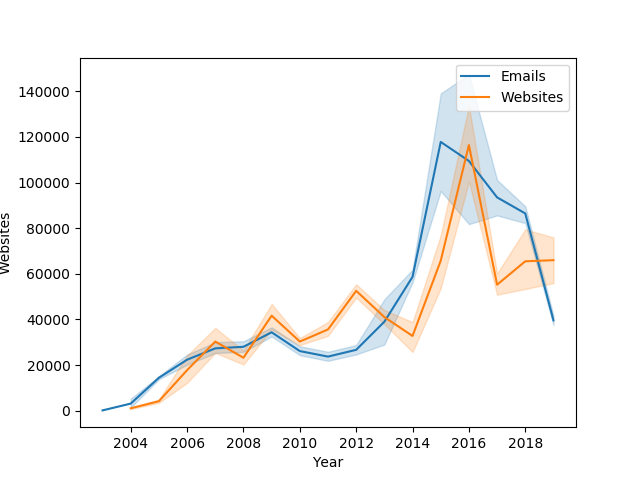
\includegraphics[width=0.49\textwidth]{apwg_attack_hist.png}
	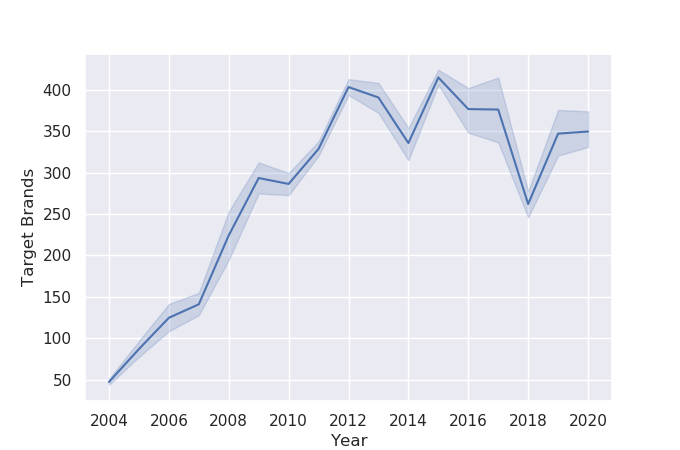
\includegraphics[width=0.49\textwidth]{apwg_brands_hist.png}
	\caption{Phishing attacks over the years (Emails, Websites and Brands
		targeted)}
	\label{fig:PHISHING_HISTORY}
\end{figure}

\section{Problem definition}
% Discuss statistics and identity theft
While the exploitation of trust or personality traits such as agreeableness or
obedience is not a new phenomenon, the internet has brought about a new
framework in which such activities can be conducted. Comparing the
aforementioned to a face-to-face setting, the former provides several advantages
for the attacker such as anonymity and a greater geographical reach. Once with
this contextual shift, the term "phishing" has been popularized. Phishing is
described as a scam by which an internet user is manipulated into disclosing
personal or confidential information that the attacker can use illicitly
\citep{MERRIAM_WEBSTER}.

In its primitive form, a phishing attack requires elementary technical
knowledge. The main skills required are the ones easily transferable from
manipulation or deceit in face-to-face interaction. This amongst other reasons
outlined in the following subsections, has contributed to the growth in
popularity of phishing attacks in the past twenty-five years.

\subsection{Current situation}
The increase in popularity of phishing is seen in the numbers registered by the
Anti-Phishing Working Group \citep{APWG} across the years. Their archives open
with the reports from 2004 adding up to 33.5 thousand unique phishing attacks
with missing data for September. After fifteen years, the APWG registered
479,468 unique phishing attacks in 2019. Besides the growth in numbers, the
aforementioned reports outline a clear advancement in the technical aspects of
the registered phishing campaigns over the years. An example of evolution is the
adoption of Transport Layer Security (TLS) used to serve phishing websites over
HTTPS. Reported usage has grown from close to zero percent in 2016, to
sixty-eight percent by the end of the third quarter of 2019 \citep{APWG_Q42019}.

\subsection{Existing solutions}
% (how do solutions deal with phishing and why is it not working) 
% https://gs.statcounter.com/
In most cases, the only source of protection against accessing phishing websites
the user has is the browser. The browser usage statistics show that Google
Chrome, Apple Safari, and Mozilla Firefox comprise 86.01\% of the market share.
All of these browsers use Google Safe-Browsing as their anti-phishing detection
system. At the surface level, this is a black-list based service which rovides
the aforementioned browsers with a list of malicious URLs through its
Application Programming Interface (API).

% Figure showing browser market share
% Look at issues with Google Safe-Browsing

Although Google Safe Browsing acts as a black-list, underneath this compilation
of malicious URLs lies an entire process of scrutinization. Based on it, the
decision-making mechanism chooses whether the URL of the studied web page should
be added to the black-list. Because of the time needed for this process to
finalize and update the list, this solution can be labeled as suboptimal. The
core issue is that attackers are quick in conducting these phishing attacks and
often go under Google Safe Browsing's radar. This is reflected in the reported
average lifespan of a phishing webpage.

The maintenance of this type of list is resource-expensive. This could be the
reason why three of the major browsers are using the same anti-phishing solution
despite its effectiveness. In conclusion, the user's main defense against
phishing is not versatile or robust enough to keep up with the speed and
sophistication of these attacks.

% ANTONIA NISOTI ET AL SHOWS THAT MOBILE BROWSERS DO NOT DELIVER THE SAME 
% PROTECTION AS DESKTOP BROWSERS
% Build an appendix of phishing attacks calendar based on APWG and point to it
%or further extract and present information


\section{Project rationale and outcomes}
% Why do this project?

% Proposed solution (What should be the level of detail?)
The trends and statistics outline the fact that phishing will remain a prevalent
type of attack for the foreseeable future. However, the protection
mechanisms of the main medium of interaction with phishing webpages are not
satisfactory, as shown by the amount of financial damage reported every year
\citep{APWG_Q42019}. Furthermore, identity theft is difficult to recover from,
and it takes time and effort.

Given the lack of empirical tests in evaluating browser protection, an
investigation of the effectiveness and accuracy of existing anti-phishing
detection systems needs to be carried out. This evaluation and research aimed at
the inner workings of these solutions serve as a starting point for developing
an improvement. As a next step, the relevant literature should be corroborated
and the most appropriate solutions stacked together and implemented. The said
implementation is meant to either outperform existing systems or complement them
to achieve an overall greater level of protection.

To the best of my knowledge, there has been no other approach structured as
described previously, which comprises the motivation of the project. There are
not many iterations of anti-phishing detection systems targeting users with
reduced technical literacy.
% TO BE REVISITED

\section{Aim and objectives}

\subsection{Aim}
The intended functional outcome of the project is a piece of software that
addresses some of the issues of phishing detection systems described in this
chapter. The first step in doing so is to develop the means to evaluate the
efficiency of Google Safe Browsing, this being the most used anti-phishing
detection system. The second step will be composed of research, design, and
development of an improved solution.

\begin{landscape}
	\begin{singlespace}
		\subsection{Objectives}
		\begin{center}
			\label{tab:OBJECTIVES}
			\begin{tabular}{ | m{0.5em} | m{18.5em} | m{23em}| m{16em} | }
				\hline
				\textbf{\#} & \textbf{Objective} & \textbf{Objective actions} &
				\textbf{Success criteria}                                       \\
				\hline
				\textbf{1}  &
				To research and develop a mechanism for evaluating the
				accuracy of phishing detection systems embedded in popular
				browsers.
				            &
				1. Research how the browser phishing detection systems and
				warnings working
				\newline\newline
				2. Find the appropriate tools and/or libraries to automate the
				process of evaluation
				\newline\newline
				2. Enter a design, development and evaluation loop until the
				automation script proves to be reliable
				            &
				The final product evaluates the phishing detection system of
				browsers with a minimal error margin.                           \\


				\hline
				\textbf{2}  &
				To  research and corroborate different anti-phishing methods
				described in the literature into a multi-layered phishing
				detection design.
				            &
				1. Research different approaches towards phishing detection
				systems
				\newline\newline
				2. Build an educated selection of features and design the
				high-level overview of the system to be implemented
				            &
				The final product evaluates the phishing detection system of
				browsers with a minimal error margin.                           \\


				\hline
				\textbf{3}  &
				To implement and calibrate a phishing detection system that
				improves the status quo and can be operated with minimal
				technical literacy
				            &
				1. Enter a software design, development, and evaluation loop to
				implement every non-machine learning feature selected in the
				research phase
				\newline\newline
				2. Train the machine learning algorithms and review their
				efficiency in carrying out the designated tasks
				\newline\newline
				3. Stack the solutions and evaluate system performance,
				efficiency, and ease of use
				            &
				The solution developed either surpasses or complements popular
				browser anti-phishing mechanisms in achieving a better success
				rate.                                                           \\

				\hline
			\end{tabular}
			\captionsetup{type=table}\caption{Objectives list}
		\end{center}
	\end{singlespace}
\end{landscape}
\section{Risk Analysis}

Considering the nature of this dissertation and the extensive amount it
plans to achieve, a risk analysis is a useful resource. This will assure a
proactive stance regarding the obstacles that are to be encountered. Besides the
resilience it offers, it helps in acknowledging areas where problems may arise
and prioritize work items based on this.

Table \ref{tab:RISK_ANALYSIS} presents the main identified risks related to
this project. Each of these has a likelihood and impact dimension attributed to
help outline the hierarchy of prioritization.

\begin{singlespace}
	\begin{center}
		\label{tab:RISK_ANALYSIS}
		\begin{tabular}{ | m{0.5em} | m{7em} | m{5em} | m{3.2em}| m{17.5em} | }
			\hline
			\textbf{\#} & \textbf{Description} & \textbf{Likelihood} &
			\textbf{Impact}
			            &
			\textbf{Intended mitigation}                                \\
			\hline
			\textbf{1}  &
			Time management issues
			            &
			Medium
			            &
			High
			            &
			Develop a plan and Gantt chart before starting the
			dissertation. Calculate the amount of time necessary to
			accomplish project's objectives and add an arbitrary
			error margin to it.                                         \\
			\hline
			\textbf{2}  &
			Sub-optimal solution results
			            &
			Medium
			            &
			High
			            &
			Allocate more time for the phishing detection system development
			than the estimated necessary. This is to calibrate and improve the
			solution's efficiency and performance                       \\
			\hline
			\textbf{3}  &
			Fatigue, anxiety or health issues
			            &
			Medium
			            &
			High
			            &
			The first two are highly influenced by time management which has
			been covered. Health issues will be prevented by following a healthy
			lifestyle and restrict interactions with contagious people. \\
			\hline
			\textbf{4}  &
			Inaccurate assumptions
			            &
			High
			            &
			Low
			            &
			Extensive research is being done at every step of the dissertation.
			This is done to reduce the number of assumptions and base the work
			only on educated ones                                       \\
			\hline
			\textbf{5}  &
			Data loss
			            &
			Low
			            &
			High
			            &
			Throughout the dissertation development, the back-up rule of 3-2-1
			will be followed. This issue dictates that three copies of the data
			should be stored on at least two mediums of storage, one being
			off-site.                                                   \\
			\hline
			\textbf{6}  &
			Chosen tools are not appropriate for the task
			            &
			Low
			            &
			High
			            &
			Do brief or comprehensive background checks for all the tools and
			libraries used in the project depending on their importance to the
			success of the project. At the same time not using more tools or
			libraries than strictly necessary                           \\
			\hline
		\end{tabular}
		\captionsetup{type=table}\caption{Risk analysis}
	\end{center}
\end{singlespace}

\section{Overview of the dissertation}
Chapter two explores the relevant literature and introduces previous work done
on the subject. Chapter three will describe the methodology used in designing
and implementing the artifact, as well as the process of developing the browser
evaluation scripts and the artifact evaluation process. Chapter four offers an
in-depth view of the requirements and requirements analysis. Furthermore, it
will illustrate the expansion fo the objectives into requirements. The fifth
chapter will follow the process of design and implementation of the artifact and
adjacent software. The last chapter will outline the outcomes of the
dissertation and close the is with a summarization of the work, presented as a
conclusion.





% =========================================================================================================
% Skipped compiling instructions
\iffalse
	\section{BU Template}
	The text within the square brackets must be deleted along with the square brackets when finalising your chapters.

	This is only a guidance template. Depending on the nature of your project, the structure of your dissertation is open to discussion. Please check with your supervisor if you are not sure.

	Arial, Normal, 11pt with 1.2 or 1.5 line spacing should be used in the main body. The text in this part has 1.5 line spacing.

	Figures must be correctly numbered with captions and paragraph text should not be wrapped around figures - same rules apply to tables. An example of figures can be found below.
	\begin{figure}[t]
		\centering
		
\includegraphics[width=0.45\textwidth]{unilogo.jpg}
		\caption{Bournemouth University}
		\label{fig:BULogo1}
	\end{figure}
	The Introduction chapter should cover the following using Heading 2 style:
	\begin{itemize}
		\item Background and context (e.g., who is your client, what is the problem, why this needs to be solved (impact), what does your client want you to do)
		\item Proposed solution (e.g., what is proposed to solve the problem) – note you should not include too many technical details, you should tell what the client is expecting from you
		\item Aims and objectives – note the SMART for objectives
		\item Success criteria – for each objective
		\item Risk analysis – a summary table must be provided with all risks and solutions.
		\item Overview of dissertation/Remaining chapters]
	\end{itemize}
\fi



%!TEX root = ../main.tex
\raggedbottom
\chapter{Background Study}
\label{chap:bgStudy}
This chapter presents a review of the research done on different aspects of
phishing. It starts by defining the research methodology used and continues with a further articulation of the issue at hand. To do so it views phishing from the attacker's standpoint and profiles the victim. For the remainder of it, the chapter presents the most relevant research done in the area and offers critical appraisal on the work it describes.

\section{Research methodology}
The subject and aim of the research and literature review shifted several times throughout carrying out the necessary work. However, the aim has constantly been to develop an in-depth and high-resolution image of the subject matter and base the work presented upon previous studies rather than suppositions. Throughout this dissertation, the systematic process used in doing the literature review is comprised of two procedures.

The first procedure dictates that the research should begin by firstly identifying a reputable and well established study. This paper is thoroughly read and the information relevant is extracted and processed accordingly.
The second procedure is used to deepen the understating of the subject. Based on the paper identified by procedure one, the points of interest are followed by spidering through the references. When the process of spidering brings in focus papers that are not relevant to the aim, the research should return to procedure one.

Following this method ensures that by the end of the research phase, there will be a clear and in-depth understanding of the status quo in the subject of interest. In addition, the papers included in this chapter have received a greater level of attention to produce a pertinent appraisal of the work they present.


\section{Understanding the popularity}

\subsection{Attacker's viewpoint}
In understanding why phishing attacks are so popular amongst attackers, it is
useful to view it from their perspective. A successful phishing attack circumvents most of a user's or enterprise's lines of defense. Most security
solutions are centered around detecting and preventing actions that have not
been explicitly initiated or allowed by the user. The key issue is that a
phishing attack, by definition, tricks the user into giving such information or
carrying out the actions intended by the threat actor.

Other appealing factors for the attacker are the inherent vulnerabilities and
proclivities of people. \cite{PRINCIPLES_OF_PERSUASION} has corroborated the
previous research on the subject to produce a list of principles of persuasion
used in phishing attacks. Looking at the first contact of the attacker with the
possible victim, namely the e-mail subject line, the study outlines that the
most popular means of persuasion employed by attackers are: Authority (32.24\%),
Strong affect (15.01\%) and Reciprocation (12.42\%). Given the amount of time
phishing attacks have had to organically evolve, we can be confident in saying
that these instruments gained popularity based on their positive influence on
the attack's success.

\begin{figure}[!b]
	\centering
	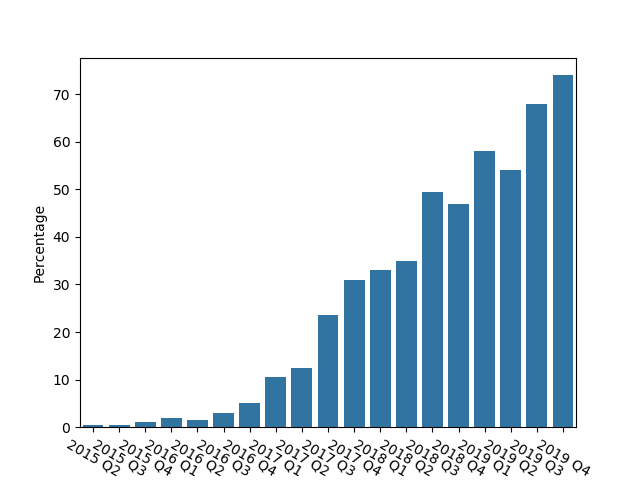
\includegraphics[width=1\textwidth]{apwg_https_usage.png}
	\caption{
		Reported number of phishing pages served over \gls{HTTPS} \citep{APWG_Q42019}}
	\label{fig:HTTPS_USAGE}
\end{figure}


\subsection{Identifying the victim}
To further the understanding of why phishing attacks are prevalent, we need to
outline the profile of the victim. A well-established study of the victim is
done by \cite{WHY_PHISHING_WORKS} which concludes the research by stating that
there is no correlation between sex, age, education, browser, operating system,
website used or hours of computer usage and the predisposition of being the victim
of a phishing e-mail. One unexpected discovery is that even in the best-case
scenarios when the subject is expecting a phishing attack, the best phishing
website deceived 90\% of the participants. The same research also describes the
elements that users look after before trusting the website, the key takeaways
being that 59\% of the participants based their decision on the page content,
with some of them (36\%) paying little attention to the address bar. The rest of
41\% based their decision on the page content and domain name, but also the
presence of \gls{HTTPS}, the padlock icon and Secure Socket Layer (\gls{SSL}) certificates.

\begin{table}[b]
	\begin{center}
		\begin{tabular}{ | m{12em} | m{12em} | m{11.5em} | }
			\hline
			                                  & \textbf{Highly susceptible} & \textbf{Less susceptible} \\ [1.25em]
			\hline
			\textbf{Age}                      & 18-24 years old or less     & 25 years old or more      \\
			\hline

			\textbf{Gender}                   & Female                      & Male                      \\
			\hline

			\textbf{Anti-phishing training}   & No training                 & Anti-phishing trained     \\
			\hline

			\textbf{Education}                & Humanities                  & Computer science          \\
			\hline

			\textbf{Training delivery method} & Non-embedded                & Embedded                  \\
			\hline

			\textbf{Personality}              & Agreeableness               & Consciousness             \\
			\hline

			\textbf{Internet usage behaviour} & E-commerce and banking      & E-mails and browsing      \\
			\hline
		\end{tabular}
		\caption{\cite{UNDERSTANDING_PHISHING_VICTIM} on susceptibility of being a victim of phishing}
		\label{tab:VICTIM_SUSCEPTIBILITY_BREAKDOWN}
	\end{center}
\end{table}

Since this research has been done, the awareness of what \gls{HTTPS} is and it's
importance has grown substantially, but so did the number of phishing websites
served using it. The launch date of the Electronic Frontier Foundation's
\citep{EFF_LETS_ENCRYPT} certificate authority which provides \gls{SSL} certificates
at no cost can be correlated to \cite{APWG_Q42019}'s reported growing adoption
in serving phishing websites over HTTPS (Figure \ref{fig:HTTPS_USAGE}). This is
especially dangerous and confusing for the victim as \gls{HTTPS} is defined as
secure Hypertext Transport Protocol \gls{HTTP} and provides the icon of a green padlock, creating the feeling of a safe and secure website.

Other studies ventured to find correlations between personality particularities and
susceptibility of being deceived by a phishing attack, but they often are in
direct contradiction. \cite{UNDERSTANDING_PHISHING_VICTIM} managed to link the
susceptibility of being deceived by a phishing attack to a set of arbitrary
characteristics. The research concluded with the description of the two extremes
of the spectrum as shown in Table \ref{tab:VICTIM_SUSCEPTIBILITY_BREAKDOWN}.

In another study, \cite{SPEARPHISHING_IN_THE_WILD} concluded that
conscientiousness is the biggest indicator of predisposition in being deceived
by a phishing attempt. This is in direct opposition to the conclusion of
\cite{UNDERSTANDING_PHISHING_VICTIM} which identifies agreeableness as the best
indicator of high susceptibility and conscientiousness as the best indicator for
low susceptibility of being a victim.


\section{Literature Review}
There is a wealth of approaches in phishing detection and prevention presented
by the literature. To better visualize them, \cite{ML_BASED_DETECTION_FROM_URL}
sinthesised the anti-phishing detection systems' literaterature structure as shown in Figure \ref{fig:PHISHING_SOLUTION_CATEGS}. In the following subsections, the discussion will be focused on software-based, as user awareness is considered out of scope for the aim of this dissertation.

The literature review is categorized in rule-based (including black-lists, white-lists and heuristics) and machine learning-based. Some of the research does have
some hybrid aspects but has been assigned to the category deemed as most
relevant. The reason behind the selected categories lies in the fundamentally
different type of classification mechanism.

\begin{figure}[t]
	\centering
	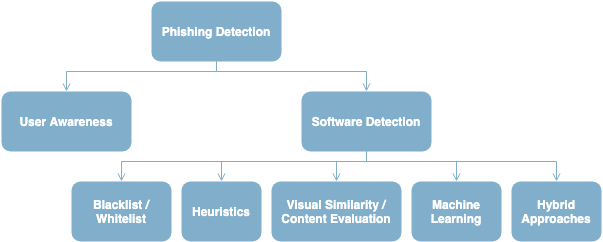
\includegraphics[width=0.9\textwidth]{phish_detection_class.png}
	\caption{
		Categorisation of phishing prevention solutions
		\citep{ML_BASED_DETECTION_FROM_URL}}
	\label{fig:PHISHING_SOLUTION_CATEGS}
\end{figure}

\subsection{Rule-based phishing detection}
\label{RULEBASED}

% (maybe speak about google safe-browsing?)

Rule-based phishing solutions classify websites as malicious or legitimate based
on a pre-defined set of rules. Because the ruleset is the centerpiece of the
detection system, the resulted performance is tightly linked to the system's
design. As a consequence, the focus is set on the selection and conditional
relationship setting.

\cite{ANTIPHISHING_AUTOMATED_WHITELIST} proposed an automated individual
white-list capable of updating itself with records of the IP addresses of each
website visited, which features a login page. If the user attempts to submit
information through such a login user interface (LUI), they get a warning
informing them that they are doing so on a webpage outside of the white-list.
The proposed solution uses the Naive Bayesian classifier to take decisions which
has delivered high effectiveness in previous studies on anti-spam
\citep{BAESYAN_KEYWORD_COMPARISON} and junk e-mail
\citep{BAESYAN_JUNK_FILTERING} filters. After the decision has been taken, the
classification is expected to be further confirmed by the user. Although the
proposed solution delivered a rate of true positives of 100\% and a rate of
false negatives of 0\%, the disadvantage is that this approach relies on the
involvement of the user, and cannot discover new phishing webpages.

Another white-list based approach is presented by
\cite{ANTIPHISHING_AUTOUPDATED_WHITELIST} which achieves phishing detection
using a two-phase method. In the proposed system the webpages are logically
split into "not visited" and "re-visited". The first module is triggered when a
page is re-visited and consists of a domain lookup within the whitelist. If the
domain name is found, the system matches the IP address to finally take the
decision. When the domain name is not recorded in the whitelist, the system uses
its second module. The second module is based on statistical analysis of the
number of hyperlinks pointing to a foreign domain used in a phishing webpage
compared to a legitimate one. After extraction, the system examines the features
from the hyperlinks to take the decision. Although the proposed system covers a
variety of phishing attacks (e.g. DNS poisoning, embedded objects, zero-hour
attack) it has declared experimental results of 86.02\% true positive rate and
1.48\% false-negative rate.

\cite{CANTINA} proposed an adaptation of the term frequency-inverse document
frequency (TF-IDF) information retrieval algorithm for detecting phishing
webpages in a content-based approach called CANTINA. The TF-IDF algorithm is
used to extract the most frequently used five words, which are then fed into a
search engine. The website's domain name is then compared with the top \(N\)
domain names resulted from the search, and if there is a match the website is
considered legitimate.
To lower the rate of false-positives, they included a set of heuristics checking
the age of the domain, the presence of characters such as '@' signs, dashes,
dots or IP addresses in the URL and some content-based checks such as
inconsistent well-known logos, links referenced and forms present. The
experimental results show a true positive rate of 97\% and a false positive rate
of 6\%. After the addition of these heuristics the false positive rate decreased
to 1\% but so did the true positive rate, which decreased to 89\%. An important
note about this research is that the resulted effectiveness is tightly linked to
the English language.

\cite{RULE_BASED_CLASSIFICATION} presents an intelligent rule-based phishing
detection system, whose ruleset is produced through data mining. The study
begins with a proposed list of seventeen phishing features derived from previous
work on anti-phishing detection systems. These are then fed into different
rule-based classification algorithms, each of which utilizes a different
methodology in producing knowledge. The conclusion presents C4.5 \citep{C4.5} as
the algorithm that produced the most effective ruleset. The extracted set is
comprised of features related to the request URL, age of domain, HTTPS and SSL,
website traffic, subdomain and multi subdomain, presence of prefix or suffix
separated by "--" in the domain and finally using an IP address. The downside of
the presented solution is the reliance on third-party services providing
information about the age of the domain, webpage traffic, and DNS record data.
Furthermore calibrating the thresholds for each feature requires complex
statistical work.

\cite{INTELLIGENT_RULE_MINING} approaches phishing detection by firstly focusing
on the extraction of key indicators that are statistically proven to be found in
phishing websites. The paper then presents a set of heuristics based on the
aforementioned statistical investigations and analysis, which are translated
into fourteen rules responsible for URL classification. Similar to
\cite{RULE_BASED_CLASSIFICATION}, the identified rules are fed into two data
mining algorithms (Apriori and Predictive Apriori), to discover effective
associations between them. The paper concluded by stating the two sets resulted
from associative rule mining, and the reported experimental accuracy of 93\%
when using the ruleset mined by the apriori algorithm. The rules used to achieve
this efficiency are presented in Table \ref{tab:APRIORI_MINED_RULES}.


\begin{singlespace}
	\begin{table}[!b]
		\small
		\begin{center}
			\begin{tabular}{ m{41.5em} }
				\hline
				\\
				\(Rule\ 1: if\ \{\ Transport\ Layer\ Security\ =\ HTTP\ \cap\ Keyword\ in\ the\ path\)

				\(portion\ of\ the\ URL\ =\ yes\ \cap\ Top\ Level\ Domain\ =\ yes\ \}\ \implies\ class\ phishing\)
				\\\\
				\(Rule\ 2: if\ \{\ Number\ of\ slashes\ in\ URL\ \geq\ 5\ \cap\ Transport\ Layer\ Security\ =\ HTTP\ \cap\ Keyword\ in\ the\ path\ of\ the\ URL\ =\ yes \}\ \implies class\ phishing\)
				\\\\
				\(Rule\ 3: if\ \{\ Special\ characters\ =\ yes\ \cap\ Transport\ Layer\ Security\ =\ HTTP\ \cap\ Number\ of\ terms\ in\ the\ host\ name\ of\ the\ URL\ > 4\ \}\ \implies class\ phishing\)
				\\\\
				\(Rule\ 4: if\ \{\ Dots\ in\ the\ host\ URL\ > 4\ \cap\ Transport\ Layer\ Security\ =\ HTTP\ \cap\ Number\ of\ terms\ in\ the\ host\ name\ of\ the\ URL\ > 4\ \}\ \implies class\ phishing\)
				\\\\
				\(Rule\ 5: if\ \{\ Number\ of\ slashes\ in\ URL\ \geq 5\ \cap\ Dots\ in\ the\ host\ URL\ > 4\ \cap\ Length\ of\ the\ URL\ > 75\ \}\ \implies class\ phishing\)
				\\\\
				\(Rule\ 6: if\ \{\ Special\ characters\ =\ yes\ \cap\ Transport\ Layer\ Security\ =\ HTTP\ \cap\ Top\ Level\ Domain\ =\ yes\ \}\ \implies class\ phishing\)
				\\\\
				\(Rule\ 7: if\ \{\ Dots\ in\ the\ host\ URL\ > 4\ \cap\ Transport\ Layer\ Security\ =\ HTTP\ \cap\ Keyword\ in\ the\ path\ of\ the\ URL\ =\ yes\ \}\ \implies class\ phishing\)
				\\\\
				\(Rule\ 8: if\ \{\ Special\ characters\ =\ yes\ \cap\ Transport\ Layer\ Security\ =\ HTTP\ \cap\ Keyword\ in\ the\ path\ of\ the\ URL\ =\ yes\ \}\ \implies class\ phishing\)
				\\\\
				\(Rule\ 9: if\ \{\ Dots\ in\ the\ host\ URL\ > 4\ \cap\ Keyword\ in\ the\ path\ of\ the\ URL\ =\ yes\ \cap\ Top\ Level\ Domain\ =\ yes\ \}\ \implies class\ phishing\)
				\\\\
				\hline
			\end{tabular}
			\caption{\cite{INTELLIGENT_RULE_MINING} rule mining results of the apriori algorithm}
			\label{tab:APRIORI_MINED_RULES}
		\end{center}
	\end{table}
\end{singlespace}

\subsection{Machine-learning based phishing detection}

Machine learning-based solutions are centered around the process of feature
extraction and selection from different parts of the website such as the URL or
HTML content, and the training of a machine learning model using this
information. This subsection will briefly discuss a variety of machine learning
approaches to anti-phishing detection systems, and the key takeaways from the
studies covered.

\cite{URL_SAYS_ALL} proposes PhishDef --- a system which does on-the-fly
classification of phishing URLs based on lexical features and adaptive
regularization of weights \citep{AROW}. The AROW algorithm offers the capability
of calibrating the classification mechanism upon making a wrong prediction. As a
result, the predictions will be of high accuracy even when the trained model is
provided with noisy data. Furthermore, PhishDef is based on an online
classification algorithm, as opposed to a batch-based one. Online classification
algorithms continuously retrain their model when encountering new data, instead
of just delivering the prediction. The accuracy of PhishDef is reported as 95\%
with an amount of noise ranging from 5\% to 10\% and above 90\% when the amount
of noise is between 10\% to 30\%. A note worth mentioning is that PhishDef
achieves the aforementioned accuracy while having low computational and memory
requirements.

Furthering the work on CANTINA mentioned in Subsection \ref{RULEBASED},
\cite{CANTINA+} enhanced the detection system by adding a feature-rich machine
learning module. The iteration is named CANTINA+, and it aims to address the
high false-positive rate of its predecessor. Besides machine learning
techniques, this enhanced iteration brings in a focus on search engines, and the
HTML Document Object Model (DOM), adding several checks on brand, domain,
hostname search and HTML attributes. Besides the inherited trade-offs of
CANTINA, the research states that one of the limitations of CANTINA+ is the
incapability of delivering predictions on phishing websites that are composed of
images, thus offering no text for it to analyze. However, while it manages to
improve upon the original implementation of CANTINA and successfully achieves an
accuracy rate of 92\%, it is still prone to producing a considerable number of
false positives.

\cite{MULTISTAGED_DETECTION_BOTNETS} presents a multi-stage detection system
that aims to both pro-actively and reactively take action against banking
bot-nets. The first feature of this model is an early warning detection module
which supervises the malicious-looking newly registered domains. The second
module does spear phishing detection using a machine learning model trained on
different variations of popular domains such as bitsquatting, omission, etc.
Although this research is geared more towards banking bot-nets, the approach
used in suspicious URL detection and spear-phishing protection is well designed
and highly relevant.

\cite{STACKED_ML_URL_HTML} takes a different approach by using a stacked machine
learning model that successfully surpasses the efficiency of single model
implementations of anti-phishing detection systems. The study shows the
comparison between the proposed stack composed of Gradient Boosting Decision
trees \citep{GBDT}, XGBoost \citep{XGBOOST}, and LightGBM \citep{LIGHTGBM} and
single models using algorithms such as support vector machine, nearest neighbor
classifier, decision trees, and random forest. Furthermore, it provides a wealth
of information about efficiency differences between different single or stacked
models. To measure inter-rater reliability for qualitative (categorical) items
and elect the best candidates for the stacking model \cite{STACKED_ML_URL_HTML}
used Cohen's kappa static \citep{DATA_MINING_T&T}. The resulted stack was
selected based on the aforementioned kappa static and the lower average error.
This method of selection lowered the false negative, false positive and false
negative rates of the stacking model when compared to all its components
individually. Finally, the research reports an accuracy rate of the stacked
model of 97.3\%. with a false positive of 1.61\% and a false negative rate of
4.46\%.

\cite{ML_BASED_DETECTION_FROM_URL} researches the possibility of a real-time
anti-phishing system, training seven different classification algorithms with
natural language processing (NLP), word vector and hybrid features. In doing so,
\cite{ML_BASED_DETECTION_FROM_URL} states the lack of a worldwide acceptable
test dataset for effectiveness comparison between phishing solutions, and
proceeds to construct one containing 73,575 URLs of which 34,600 legitimate and
37,175 malicious. The paper uses this dataset to conduct comparisons between
previous work in the field and the selected classification algorithms (Decision
Trees, Adaboost, Kstar, K-Nearest Neighbour, Random Forest, Sequential Minimal
Optimization and Naive Bayes), outlining the best performers. The most effective
combination discovered is the Random Forst algorithm trained with NLP features.
It achieved an experimental accuracy of 97.98\% in URL classification, while
being language and third-party service independent, and achieving real-time
execution and detection of new websites. An important tendency emergent from the
comparisons is that the NLP features seem to improve accuracy across the
majority of machine learning algorithms covered.

\begin{singlespace}
	\small
	\begin{center}
		\label{tab:EXISTENT_SOLUTIONS}
		\begin{tabular}{ | m{8em} | m{13em} | m{8.5em} | m{2.3em} | m{5em} | }
			\hline
			\textbf{Plugin for Phishing} & \textbf{Features \& Techniques}       & \textbf{Browser}    & \textbf{Acc \%} & \textbf{Service  type} \\
			\hline
			GoldPhish                    & Heuristics \& Features-based          & IE                  & 98              & Free                   \\
			\hline
			Cloudmark                    & Heuristics                            & IE                  & 94              & Free                   \\
			\hline
			MS SmartScreen               & Blacklist and whitelist               & IE                  & 95.9            & Free                   \\
			\hline
			Netcraft (Customise)         & Blacklist and whitelist               & Chrome, Firefox     & 90              & Free                   \\
			\hline
			SpoofGuard                   & Heuristics \& Features-based          & IE                  & 91              & Free                   \\
			\hline
			Phishdentity                 & Google search-by-image API            & IE                  & 97.2            & Research               \\
			\hline
			PhishTackle                  & Heuristics \& Features-based          & IE                  & 91.3            & Research               \\
			\hline
			PhishGuard                   & Heuristics                            & Firefox             & 94              & Research               \\
			\hline
			PhishIdentifier              & Heuristics                            & Firefox             & 92              & Research               \\
			\hline
			PhishTester                  & Heuristics \& Features-based          & IE                  & 97.1            & Research               \\
			\hline
			CANTINA+                     & Heuristics \& Features-based          & IE                  & 98.06           & Research               \\
			\hline
			PhishAri                     & Features-based                        & Chrome              & 92.52           & Research               \\
			\hline
			PhishShield                  & Heuristics \& Feature-based           & Chrome              & 96.57           & Research               \\
			\hline
			PhishNet                     & Blacklist                             & Chrome              & 95              & Research               \\
			\hline
			PhishDef                     & Heuristics \& Feature-based           & Chrome              & 97              & Research               \\
			\hline
			Google Safe Browsing         & Blacklist                             & Chrome, Firefox     & 93.3            & Free                   \\
			\hline
			PhishZoo                     & Heuristics                            & Chrome              & 96.10           & Research               \\
			\hline
			Seclayer                     & Heuristics                            & IE, Chrome          & 91              & Free                   \\
			\hline
			IPDPS                        & Heuristics \& Feature and image based & IE, Chrome, Firefox & 98.55           & Research               \\
			\hline
		\end{tabular}
		\captionsetup{type=table}\caption{A comparison of existing solutions \citep{INTELLIGENT_PHISHING_ANFIS}}
	\end{center}
\end{singlespace}

\cite{INTELLIGENT_PHISHING_ANFIS} studies the performance of a few machine
learning models, one of which is an artificial neural network named Adaptive
Neuro-Fuzzy Inference System \citep{ANFIS} when trained with integrated text,
image, and frame features. Before venturing to do so, the research presents a
brief comparison between the proposed solution, and numerous other anti-phishing
detection systems which can be found in Table \ref{tab:EXISTENT_SOLUTIONS}.
Throughout its content, the paper builds a set of 35 features from phishing
websites analysis and related work and compares their efficiency. These are then
bound in sets and fed into ANFIS, SVM, and KNN algorithms to study the outcome.
The ANFIS-based hybrid solution (including text, image and frame features)
delivered an accuracy of 98.30\%. Although the research considers the previously
mentioned solution as the conclusion, the ANFIS text-based classification
records an accuracy of 98.55\%. Besides this, throughout the study, there is
evidence that text-based detection systems tend to outperform image-based,
frame-based and hybrid ones.

\cite{SVM_ANTI_PHISHING} presents a solution based on a selection of seventeen
web content features which are fed into a Support Vector Machine (SVM) learning
algorithm. The most effective features are elected based on accuracy, error,
Cohen's Kappa Static \citep{DATA_MINING_T&T}, sensitivity, and the F-Measure
\citep{DATA_MINING_T&T}. Before evaluation, the features are fed into the SVM
algorithm to extract knowledge in the form of rules to increase
comprehensibility. By doing this, the importance and effect of each feature can
be extracted. The research benchmarks the features and discusses the
consequences of omitting different rules, outlining the ones with the biggest
contribution in making a correct prediction.
By using this approach the study reports an impressive experimental result of
99.14\% accuracy, with only 0.86\% false negative. Furthermore, the proposed
solution achieves zero-day phishing detection and language independence while
maintaining independence from search engines and third party services.

Finally, \cite{SVM_SIMILARITY_INDEX} focused on studying how similarity indexes
influence the accuracy of support vector machine models, the aim being the
production of a lightweight anti-phishing detection system, suitable for devices
such as smartphones. The paper first presents a set of base URL features
composed of number of hyphens, number of dots, the number of numerical
characters and IP presence. To this set \cite{SVM_SIMILARITY_INDEX} added the
classic Levenshtein distance, normalized Levenshtein distance, Jaro Winkler
distance, the longest common subsequence, Q-Gram distance, and the Hamming
distance individually, and measured the influence by comparing it to the base
accuracy. All the aforementioned additions calculate the similarity index
between two strings. This calculation is done on the entire database of two
thousand records which is incorporated in the proposed solution (1000 legitimate
URLs and 1000 malicious). The study concludes by reporting an accuracy of 95\%.
Furthermore, it states that the Hamming distance is the most effective from the
studied set, improving the overall recognition rate by 21.8\%.

\subsection{Google Safe Browsing}
As previously stated, Google Safe Browsing is responsible for protecting the top three browsers in terms of popularity: Google Chrome, Apple's Safari and Mozilla Firefox. Because of this, the artefact produced throughout the present dissertation is aiming to surpass it's performance. This subsection introduces Google Safe Browsing in a brief manner, after which presents work conducted to assess it's effectiveness.

\cite{GOOGLE_SAFE_BROWSING_VERSIONS} describes the mechanism behind Google Safe browsing and captures the differences between the different API versions. However, the study dates back to 2015, so the version comparision table includes only the first three versions. Since then, version four has been released, marking the end of support for version two and three.
\cite{GOOGLE_SAFE_BROWSING_V4} doesn't mention any fundamental changes to the API, but details the update in the focus towards the growing mobile. To adapt to this, the new API is optimized towards the challenges of the mobile environment: the limited power, network badwidth and poor quality of service. Furthermore, the protection per bit is maximized, due to cellular data being a direct expense of the user.

\begin{singlespace}
	\small
	\begin{center}
		\label{tab:OPTIMISED_MODELS}
		\begin{tabular}{ | m{13em} | m{12.9em} | m{13em} | }
			\hline
			\textbf{Version 1}                     &
			\textbf{Version 2}                     &
			\textbf{Version 3}                                                                                                                     \\
			\hline
			The hashing algorithm used in this
			version is MD5.                        & The hashing algorithm used in this
			version is SHA 256.                    & To improve the efficiency, protocol buffers are
			used by encoding the chunk data.                                                                                                       \\
			\hline
			The efficiency is less and it is not
			scalable.                              & In the place of a single versioned
			list, a series of "chunks” is used.    & Host keys are not used.                                                                       \\
			\hline
			-The entire phishing list entries are to be
			downloaded at once because the
			partial list updates are not supported
			till the time the user fully downloads
			the recent version of list.            & A list of URLs is received when the
			list of chunks is communicated
			while updating.                        & Optional metadata was included in HTTP
			Response for Full-Length Hashes .                                                                                                      \\
			\hline
			The phishing data is given to the client in
			an order from old to new. For the
			phishing sites it is inefficient as they
			have a short lifetime.                 & The Chunks present are 32-bit
			truncated hashes                       & To differentiate between the kinds of sites and
			to allow more warnings, metadata
			functionality was used by Google-malware-
			shavar list.                                                                                                                           \\
			\hline
			As regular updates are required, so the
			bandwidth consumption is escalated.    & As soon as a match is discovered,
			the 32 bit chunk is
			communicated to Google and in
			return a list of 256 bit hash is
			acquired.                              & For the full hash, modifications are carried out
			in the cashing semantics.                                                                                                              \\
			\hline

			It is time consuming as the users scarcely
			find a match with the present pattern. & As compared to version 1, it is
			faster                                 & An expiration time is included in the HTTP
			Response for Full-Length Hashes in
			response                                                                                                                               \\
			\hline

			It is slow and has high latency.       & It has improved speed and reduced
			Latency.                               & When an update request is sent, each time the
			clients are required to wash off cashed full
			length hashes                                                                                                                          \\
			\hline
			                                       &                                                  & Message Authentication Code (MAC) support
			is eliminated.                                                                                                                         \\
			\hline
			                                       &                                                  & The API key format is modified. The Google
			Developers Console manages the API keys.                                                                                               \\
			\hline
		\end{tabular}
		\captionsetup{type=table}\caption{A comparison of existing solutions \citep{INTELLIGENT_PHISHING_ANFIS}}
	\end{center}
\end{singlespace}


\begin{figure}[t]
	\centering
	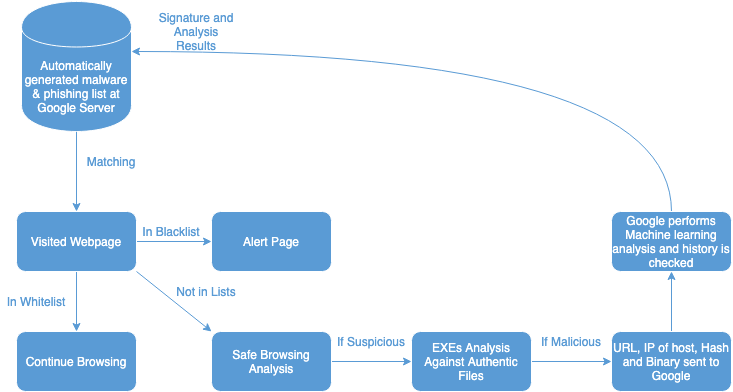
\includegraphics[width=0.95\textwidth]{google_safe_browsing.png}
	\caption{
		Categorisation of phishing prevention solutions
		\citep{ML_BASED_DETECTION_FROM_URL}}
	\label{fig:PHISHING_SOLUTION_CATEGS}
\end{figure}

Moving to performance assessment, \cite{SECURITY_BUSTERS} presents a thorough evaluation of anti-phishing detection systems embedded in different browsers and on different platforms. In developing the proposed proof of concept security proxy, \cite{SECURITY_BUSTERS} uncovered the classification accuracy issues of popular browsers. The study compiles information on the substantial difference between phishing URL detection and malicious URL detection (Table REF). It is noticeable that from all the browsers that use GSB, Google Chrome is the better performer.

\begin{singlespace}
	\begin{center}
		\label{tab:OPTIMISED_MODELS}
		\begin{tabular}{ | m{12em} | m{12em} | m{11.5em} | }
			\hline
			                                 & \textbf{True positives} & \textbf{False negatives} \\
			\hline
			\textbf{IE (Windows)}            & 48.4\%                  & 9.9\%                    \\
			\hline
			\textbf{Opera (Windows)}         & 77.9\%                   & 8.4\%                    \\
			\hline
			\textbf{Chrome (Windows)}        & 93.0\%                   & 1.3\%                    \\
			\hline
			\textbf{Firefox (Windows)}       & 86.7\%                   & 5.9\%                    \\
			\hline
			\textbf{Opera mobile (Android)}  & 75.9\%                   & 7.9\%                    \\
			\hline
			\textbf{Firefox mobile(Android)} & 85.4\%                   & 3.4\%                    \\
			\hline
			\textbf{Safari mobile (iOS)}     & 38.7\%                   & 26.4\%                    \\
			\hline
		\end{tabular}
		\captionsetup{type=table}\caption{A comparison of existing solutions (The missing percentages mark phishes that went offline during testing) \citep{INTELLIGENT_PHISHING_ANFIS}}
	\end{center}
\end{singlespace}

\section{Chapter overview}
This chapter outlined the status quo of the relevant literature, expanding on
the key takeaways of each study presented. As shown, the subject of phishing is
not only prevalent in the field of security, but in psychology and others as
well. The features and mechanisms considered as most effective by the studies
presented in the rule-based and machine learning-based solutions will shape the
design of the artifact.

% Background study should have between 10 and 30 papers

%[REVISIT SECTION AND GO INTO DETAIL]


% Machine learning based phishing detection from URLs
% An AI-based multi-stage detection system of banking botnets
% Intelligent web-phishing detection and protection scheme using integrated features of images, frames and text
% A comparison of Machine learning techn iques for phishing detection

%\section{Hybrid phishing detection systems}

%Hybrid phishing detection systems emerged as a natural inclination to gather the best of different categories of solutions. The strategy of combining classifiers of different nature has achieved impressive results, often surpassing the efficiency and accuracy of single category classifiers.




%A stacking model using URL and HTML features for phishing webpage detection
%GET REFERENCES FROM THE PAPER ABOVE and end with CONCLUSION

% Do an overview of research based on zero-hour protection and percentage of success





% =========================================================================================================
% Skipped compiling instructions
\iffalse
	\section{Template Text}
	Figures must be correctly numbered with captions and paragraph text should not be wrapped around figures - same rules apply to tables. An example of figures can be found below.
	\begin{figure}[t]
		\centering
		
\includegraphics[width=0.45\textwidth]{unilogo.jpg}
		\caption{Bournemouth University}
		\label{fig:BULogo2}
	\end{figure}
	You should always start with an overview (Heading 2 style) to tell what this chapter is about and finish with a summary (Heading 2 style) to tell what has been covered in this chapter.

	The Background Study (Research) or State of Art chapter is to provide your readers with information that they cannot be expected to know in detail but which they will need to know in order to fully understand and appreciate the rest of the dissertation. In short, it describes the research you have done in order to prepare for the project. You should use this section to demonstrate how much you really understand the problem domain in terms of previous (related) literature and existing solutions. For example, if your project is about developing a bespoke online CRM system for a client, this section is expected to answer the following questions:
	\begin{enumerate}
		\item What is CRM (Customer Relationship Management)?
		\item What are the characteristics of CRM?
		\item What are the main types/models of CRM?
		\item How CRM is usually implemented and what should be considered in the implementation?
		\item Are there any existing solutions and what are their advantages and limitations?
	\end{enumerate}

	\subsection{Literature Review}
	Note Literature Review is not often used as the title of this chapter even if your project is research based
\fi

%!TEX root = ../main.tex

% Judgement and analysis in planning: Mature analysis and judgement in planning showing flexibility and high awareness of contingencies, efficiency and monitoring. Fully comprehensive risk analysis and contingency planning

% Analysis of the problem: Full consideration has been given to analysis alternatives and an entirely appropriate and effective analysis of the problem results. Depth in judgement and final choices, and effective reativity in analysis

% Selection and justification of processes, methods and tools: Real depth of insight is shown, with discerning judgement in final choices, demonstrating unusual insight and very effective, creative approach to the project. Methods/technology are totally appropriate to the objectives, with a thorough, considered justification for their selection, and are used with flair.

% Appropriateness of solution design: Full consideration has been given to design alternatives and an entirely appropriate and effective solution results. Real depth of insight is shown, with discerning judgement in final choices, demonstrating unusual insight and very effective creativity in designing a solution to the problem that is as close to an optimum solution as can be expected.

% Appropriateness of evaluation design: Full consideration has been given to evaluation alternatives and an entirely appropriate and effective evaluation approach results. Real depth of insight is shown into the factors affecting the quality of the solution, with discerning judgement in final choices, demonstrating unusual insight and very effective creativity in designing effective evaluation at all stages of development.
\chapter{Methodology}
\label{chap:methodology}

To ensure transparency and reproducibility of the outcomes, this chapter articulates the methodology used in the organizational, structural and procedural aspects of the dissertation. Firstly, it introduces the process of initial analysis and planning that sets the base for the present work. After this, it describes the methodology used in carrying out the research and literature review. The following subsection shows insight into the process of translating objectives into requirements and the design decisions taken. The penultimate subsection will discuss the technical details of the artifact. It will increase the resolution at which the design has been presented. Finally, the last subsection will expand over the methodology of evaluation used throughout this dissertation.

\section{Planning and initial analysis}
A compulsory prerequisite of the planning and initial analysis phase is problem definition. The low-resolution problem definition developed at this stage serves as the cornerstone for further design and analysis. After the problem definition is produced, research is carried out to confirm its existence and particularities. This is done to reduce the discrepancy between the subjective view on the problem and its objective state defined by the literature.

From research on the problem of phishing and how it's impact maps on different areas, a formal compilation of objectives has been extracted as shown in Table \ref{tab:OBJECTIVES}. The next stage is designing a bare but viable solution specification around the aforementioned objectives. Based on this specification, the necessary research and procedures identified and mapped over a Gantt chart with an educated time estimate attributed to each. The final step of the initial analysis and planning is to perform a risk analysis. This reduces the probability of confronting an obstacle that has not been identified, thus having no planned mitigation.

To better visualize the planning and initial analysis phase, an illustration of the sequence of procedures is presented in Figure \ref{fig:INITIAL_ANALYSIS}.

\begin{figure}
	\centering
	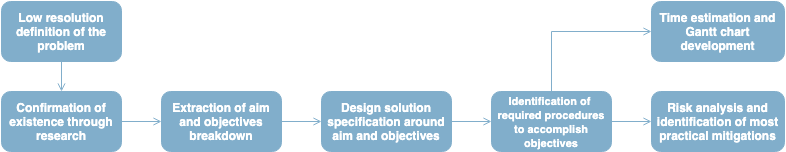
\includegraphics[width=1\textwidth]{initial_analysis.png}
	\caption{Illustration of initial analysis}
	\label{fig:INITIAL_ANALYSIS}
\end{figure}

\section{Research methodology}
The target of the research and literature review shifted from one chapter to another. However, the aim has constantly been to develop an in-depth and high-resolution image of the subject matter and base the work presented upon previous studies rather than suppositions. Throughout this dissertation, the systematic process used in doing the literature review is comprised of two procedures.

The first procedure dictates that the research should begin by firstly identifying a reputable and well established study. This paper is thoroughly read and the information relevant is extracted and processed accordingly.
The second procedure is used to deepen the understating of the subject. Based on the paper identified by procedure one, the points of interest are followed by spidering through the references. When the process of spidering brings in focus papers that are not relevant to the aim, the research should return to procedure one.

Following this method ensures that by the end of the research phase, there will be a clear and in-depth understanding of the status quo in the subject of interest. In addition, the papers included in the background study have received a greater level of attention to produce a pertinent appraisal of the work they present.

% DESING-OLD: The second step is the identification of highly performant machine learning-based solutions and the study of their design. Most of the research on anti-phishing detection systems presents comparisons of the inner workings of the proposed solution with other related implementations. Based on these, the set of the most effective mechanisms identified can be implemented to work together towards classifying URLs. Besides this, the experimentation phase includes the training of different machine learning models, calibrating parameters, changing training data, and the comparison of results. 
% It's design is built and refined through a loop of research and experimentation

\section{Artefact design and development}
The functional outcome of this dissertation is composed of two artifacts. The first is the Google Safe Browsing evaluation tool used to uncover Safe Browsing's classification accuracy. This tool will perform evaluation using both the browser in a realistic scenarion and the Google Safe Browsing API. The second artifact is the classifier used to predict whether an URL points to a phishing page or not.

\subsection{Evaluation tool}
The evaluation tool is written in Python and uses the Selenium framework for browser automation. Python is used due to it's extensive support and ease of use. The selenium framework is chosen because of it's reputation in browser automation testing and expansive documentation. The target of the evaluation tool is to mimic a user clicking on a phishing link. This is done in order to capture effectiveness in a real-world scenario. The alternative to this is using Google's Safe Browsing API for checking.

The URLs used in the evaluation process are the latest provided by Phishtank at the moment of evaluation. These are confirmed to be online and malicious by the PhishTank community. The test executed for each of the malicious URLs starts with loading the default profile of the Google Chrome user. Experimentation with the browser has shown that not loading a user's profile delivers unreliable results. After doing so the URL is opened and the page shown by the browser is studied. When a page is classified as malicious, the browser displays a custom page with a warning as shown in Figure \ref{fig:PHISHING_PREVENTED}. To verify whether the browser correctly classifies the URL, the tool searches the page's source code for Google's license details present in the warning page. If the browser shows the warning page overlay, the classification is marked as a true-positive, otherwise it is recorded as a false-negative.

\begin{figure}
	\centering
	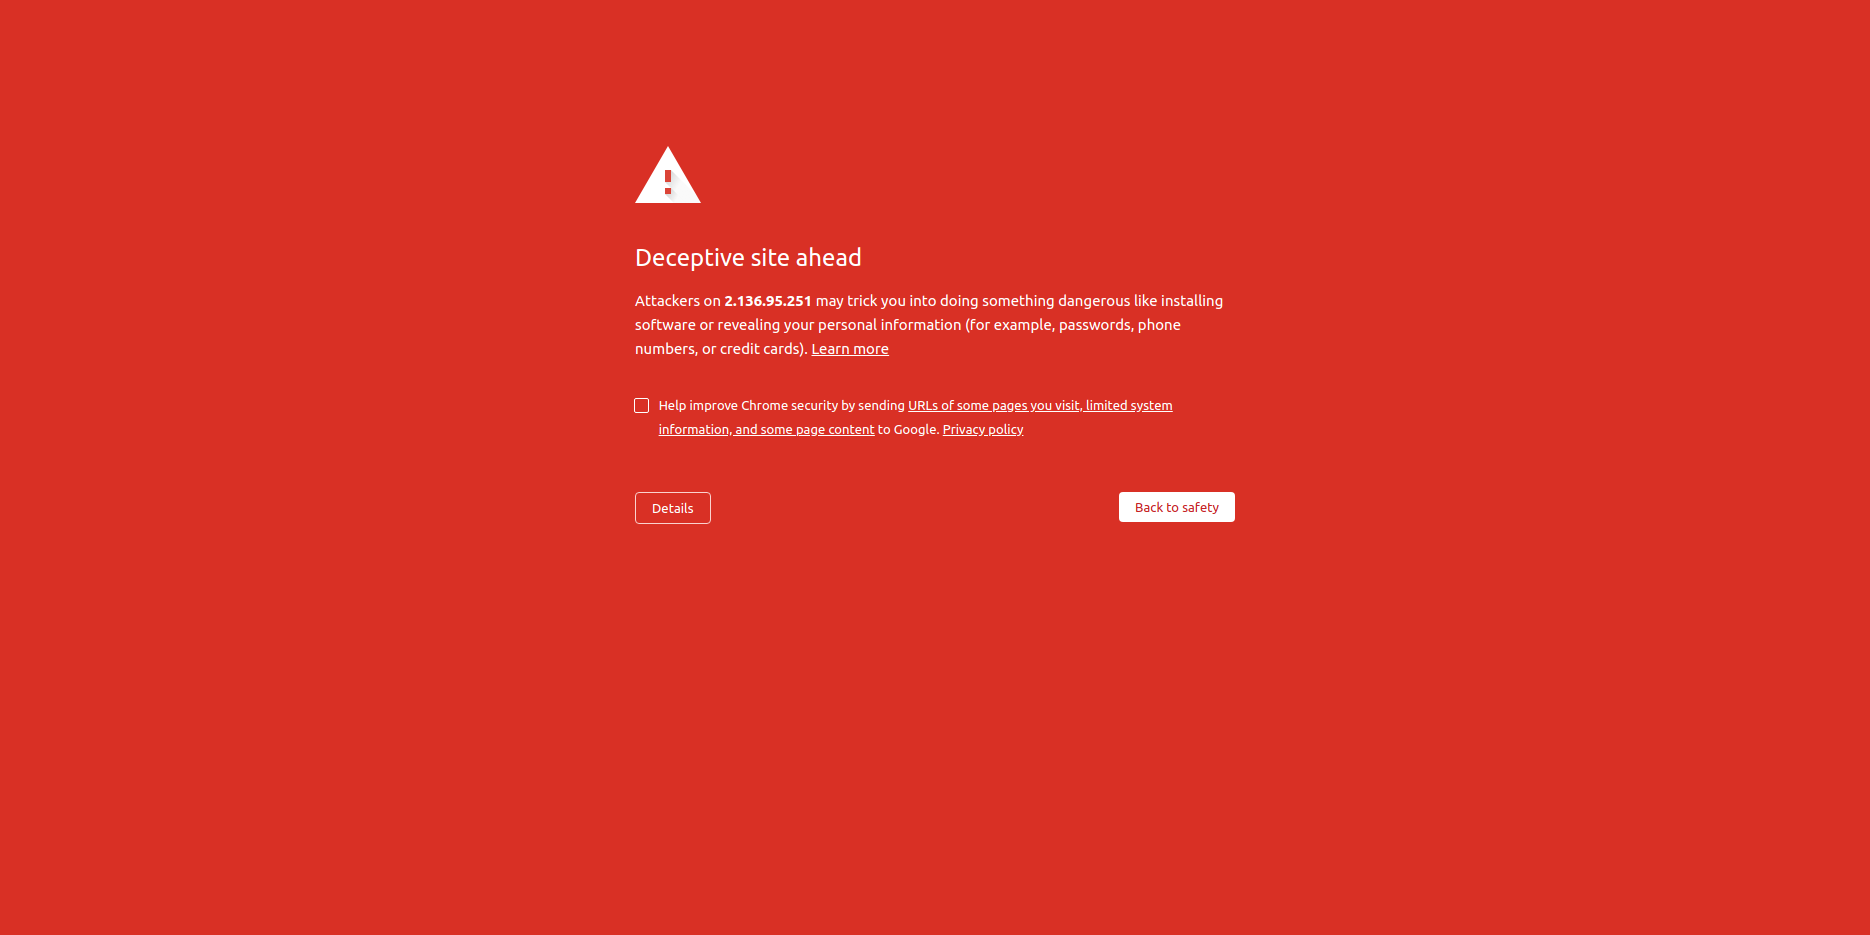
\includegraphics[width=1\textwidth]{malicious.png}
	\caption{Example of browser's warning page overlay}
	\label{fig:PHISHING_PREVENTED}
\end{figure}

\subsection{The classifier}
The classifier is the main artefact, set to accomplish the dissertation's aim of delivering better protection against phishing than the most popular browsers do. The selected approach in designing a competitive anti-phishing detection system is through the identification of key performance indicators that are efficient in phishing URL classification. Naturally, the first step in designing the artifact is corroborating information from a wide range of studies on the indices that achieve high classifications accuracy. Following this, the algorithms are compared and the best performing one is selected
Given the multi-layered structure of the artifact, each layer has it's own implementation specification and is discussed separately.

%SPEAK ABOUT PARAMETERS AND DATASET

The machine learning models compared in this dissertation are trained using Python and SciKitLearn library. Python is chosen over other programming languages as it is considered the de-facto in the field of data science. The SciKit library is used as an abstraction of the actual machine learning algorithms. By alleviating the complexity of the implementation of machine learning algorithms used, the saved time is allocated towards experimentation and calibration.

The wrapper and the set of additions are implemented in using the same programming languange. Although better performance can be achieved using a different languange, this is done to preserve continuity throughout the artefact.

TO BE REVISITED
%The development lifecycle

\section{Evaluation methodology}
The evaluation of browser's anti-phishing detection mechanism is done in two phases. Firstly the browser will be assessed using newly discovered phishing URLs. After a week of the aforementioned evaluation, the browser will be assessed again using same data. The rationale behind this lies in the study of how browsers evolve their defenses regarding old phishing data.

The evaluation of the machine learning models is based on a set of metrics that cover all the performance areas. In addition to covering performance areas, the proposed set makes the process of identifying flaws in callibration easier. Besides these, the evaluation methodology will coincide with the one presented by some of the studies discussed in the backgroud study. This is done with the aim of achieving consistency and offering a fair comparison with existent work.\newline


\begin{equation}
	\label{eq:PRECISION}
	Precision = \frac{TP}{TP+FP}
\end{equation}
\begin{equation}
	\label{eq:SENSITIVITY}
	Sensitivity = \frac{TP}{TP+FN}
\end{equation}
\begin{equation}
	\label{eq:FMEASURE}
	F-Measure = 2*\frac{Precision * Sensitivity}{Precision + Sensitivity}
\end{equation}
\begin{equation}
	\label{eq:ACCURACY}
	Accuracy = \frac{TP+TN}{TP+TN+FN+FP}
\end{equation}
\newline

The metrics presented in \ref{eq:PRECISION},\ref{eq:SENSITIVITY},\ref{eq:FMEASURE} and \ref{eq:ACCURACY} represent key statistical concepts. A system is said to be precise (\ref{eq:PRECISION}) when it delivers a high level of correct prediction values. . Sensitivity \ref{eq:SENSITIVITY}, also known as recall, outlines system's predisposition in classifying an legitimate URL as being malicious. As the system grows in sensitivity, it reduces the number of false-negatives it produces. To put things in perspective, precision is the ratio between all adequate classification errors and all classification errors, whereas recall is the ratio of all classification errors and all existing errors.
The F-Measure (\ref{eq:FMEASURE}) is the harmonic mean of precision (the number of correct predictions) and robustness (works well with URLs difficult to classify). It is a composed metric which penalizes the extreme values and is meant to provide a single measurement for a system which illustrates the level of optimization. Finally, the accuracy (\ref{eq:ACCURACY}) measures the ratio of true-positives and true-negatives.

% TODO: Fill in with explanation
In addition to the aforementioned metrics, the Receiver Operating Characteristic (ROC) curve

The final evaluation of the produced classifier is done in comparison to the evaluation tool's results. It is based on the same data set and metrics to eliminate any variables that may appear between evaluation methods.

% =========================================================================================================
% Skipped compiling instructions
\iffalse
	1st module Whitelist/Blacklist
	Hash urls and do lookups as cheap as possible
	2nd module Heuristics
	Compile a set of heuristics from the papers based on performance
	3rd module Visual similarity/Content evaluation
	Think about studying the visual similarity or some content evaluation if feasible
	4th module Machine learning
	use Cohen's kappa static to measure agreement between stacked machine learning algos
	URL classifier (supervised learning)
	Domain classifier (trained with https://github.com/elceef/dnstwist)
	DGA classifier (optional)

	Figures must be correctly numbered with captions and paragraph text should not be wrapped around figures - same rules apply to tables. An example of figures can be found below.
	\begin{figure}[t]
		\centering
		
\includegraphics[width=0.45\textwidth]{unilogo.jpg}
		\caption{Bournemouth University}
		\label{fig:BULogo3}
	\end{figure}
	You should always start with an overview (Heading 2 style) to tell what this chapter is about and finkish with a summary (Heading 2 style) to tell what has been covered in this chapter.

	This chapter is about discussing your project planning and methodology. Note that your chosen methodology should be based on the constraints and complexity of your project instead of some common senses with no link to your own project.]
\fi

%!TEX root = ../main.tex

\chapter{Implementation}
This chapter follows the process of producing and optimising the artefact to fulfill the previously articulated objectives. The first section of the chapter follows the research on Google Safe Browsing's effective in detecting phishing websites. The accuracy target of the classifier implemented in this chapter is bounded by the results of the aforementioned case study. 

The next section explores different machine learning algorithms and URL features, aiming to deliver satisfactory results in comparison with the threshold. After this, a number of features that could complement the machine learning solution are presented and assessed. Finally the classifier is brought together and assessed as a whole.

\section{Threshold definition}
Before attempting to improve the level of protection the most popular browsers offer, the system's effectiveness needs to be assessed. In doing so the behaviour of the user will be simulated using an browser automation framework in accessing confirmend phishing websites. The outcome of this serves as an accuracy threshold for the proposed artefact.

The first step of the process is data aquisition. A list of URLs pointing to online phishing webpages, confirmed to be malicious by the PhishTank community is fetched from their archive. The first test is run on the data available on the 1st on April. Testing a total number of 9345 phishing URLs, Google Safe-Broswing managed to achieve a total accuracy of 50.76\%. 
The next test is run with the data published on the 7th of April. This time Google Safe-Browsing performed slightly worse reporting an accuracy of 48.32\% on the 8164 phishing URLs. Running the same test on the data aquired on the 1st of April shows a significant drop in accuracy, reporting an accuracy of 40.28\% on a number of 9359 URLs.

Upon a surface level inspection it is noticeable that given it's popularity in usage, Google Safe-Browsing influences the lifetime of a portion of phishing URLs. It is probable that attackers adapt to the situation and remove phishing webpages detected, or serve them through different URLs. Moving a webpage from one domain to another is not resource expensive and allows the attackers to dodge the browser's anti-phishing detection system.

Finally, the threshold is set to be the highest accuracy recorded across the two tests of 50.76\%.

\section{List based module}

It is safe to assume that most of web browsing activity takes place across a limited set of domains. This is reflected in different rankings of most popular domains. Because these are known to be benign, there is no use in wasting resources on classifying them. This is reasoning behind the inclusion of a list based module in the phishing detection system to be developed.
The white-list included is comprised of the domains ranking published by \cite{MAJESTIC_MILLION}.

\section{Machine learning module}
A pattern in effective anti-phishing detection systems is the use of machine learning. A well developed module of this kind increases the performance and robustness of the proposed artefact. Besides this, it offers the capability of dealing with newly registered phishing domains and URLs.

\subsection{Algorithm selection}
The first step in building this module is the selection of machine learning algroithms. The set used is based on the emergent pattern of algorithms used in the Background Study (\ref{chap:bgStudy}) and is composed of Naive Bayes, Decision Tree, Random Forest, Support Vector Machine. In addition to these, the multilayered perceptron neural network is added with the purpose of experimentation.

\subsection{Experimentation and calibration}
The starting set in feature selection is based on the work of \cite{SVM_SIMILARITY_INDEX}. It's reported accuracy far surpasses the threshold and it makes use of similarity indexes. These similarity indexes are highly relevant as most phishing URLs try to decieve the victims by including different variations of the target brand or domain.

The first feature selected is URL length. Most of the literature acknolowdges the difference in URL length between legitimate and phishing URLs. One example is illustrated in \cite{STACKED_ML_URL_HTML} (Figure \ref{fig:URL_LENGTH_DISTRIBUTION}), showing the distribution over a set of 50,000 URLs.

\begin{figure}[t]
	\centering
	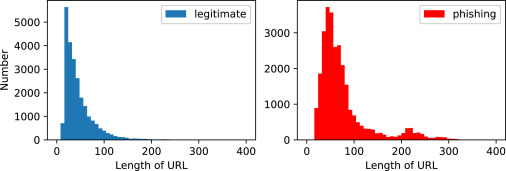
\includegraphics[width=0.9\textwidth]{url_length_50k.jpg}
	\caption{URL length distribution over a dataset of 50,000 records}
	\label{fig:URL_LENGTH_DISTRIBUTION}
\end{figure}

The second feature chosen is the number of hyphens. It is common for phishing URLs to use such characters to deceive the victim by chaining the target brand using hyphens (e.g. www.example-secure-bank.com).

The third feature is the number of dots. This is used in a simmilar manner as hyphens are, only it allows for using subdomains to create the illusion of the legitimate page (e.g. www.example.secure.bank.com)

The fourth feature is the number of numerical characters present in the domain. This is included because it is uncommon for legitimate domains to contain any numerical characters.

The fifth is the presence of an IP address in the URL. Although substantially less prevalent in current phishing attacks, it still happens that some of the phishing URLs are not addressed by domain name, but by IP address. This is a solid indicator that the URL may point to a phishing webpage.

The last feature is the Hamming distance between the URL to be classified and a top N benign domains. Similarity indexes like the Hamming distance calculate the distance of two pieces of data, in this case the distance between two strings of characters. It does so through a mathematical formula which outputs 0 or 100 on identical strings depending on implementation. For the first test the algorithm is trained with the maximum hamming distance between the input URL and top 1000 benign domains from the \cite{MAJESTIC_MILLION} dataset.

\begin{figure}
	\centering
	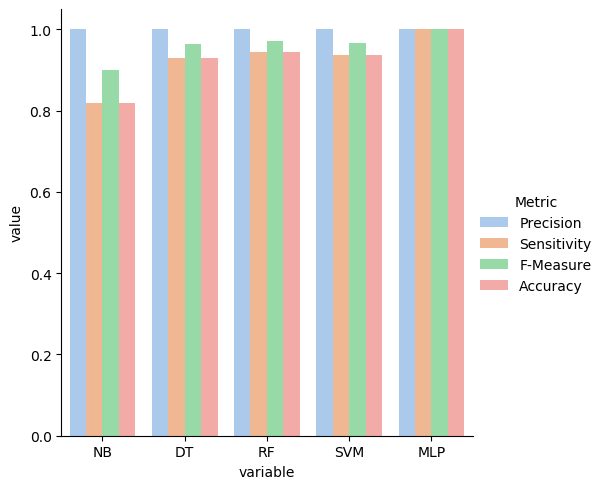
\includegraphics[width=0.49\textwidth]{hamming5k_on_phishtank_0401.png}
	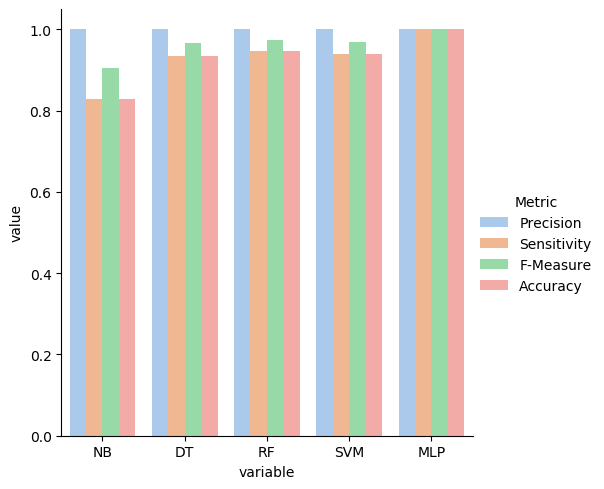
\includegraphics[width=0.49\textwidth]{hamming5k_on_phishtank_0405.png}
	\caption{URL length distribution over a dataset of 50,000 records}
	\label{fig:HAMMING_ON_PHISHTANK}
\end{figure}

The results of this feature compilation are far exceeding Google Safe-Browsing's accuracy. However when the models are evaluated on a dataset that includes benign URLs the metrics show a significant drop in every aspect exept sensitivity. Figure \ref{fig:HAMMING_ON_MIXED} illustrates the bias of the model towards classifying URLs as malicious on a 5,000 records dataset (left side) and a 25,000 dataset (right side). Both the datasets are composed of half benign urls, half malicious.

\begin{figure}[b]
	\centering
	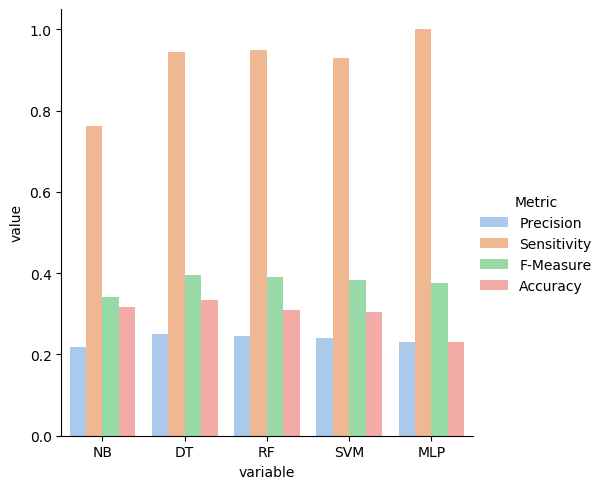
\includegraphics[width=0.49\textwidth]{hamming5k_on_mixed.png}	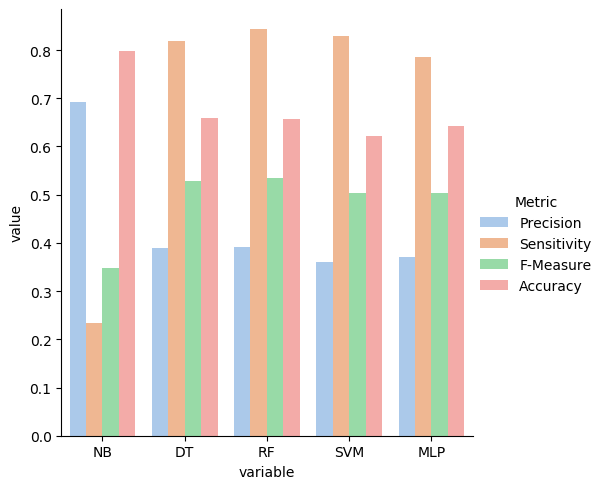
\includegraphics[width=0.49\textwidth]{hamming25k_on_mixed.png}
	\caption{URL length distribution over a dataset of 50,000 records}
	\label{fig:HAMMING_ON_MIXED}
\end{figure}

These results differ from what is reported by \cite{SVM_SIMILARITY_INDEX} because the models are trained on different datasets. Given the circumstances, the next step is improving the accuracy and lower the sensitivity by tweaking the features. The aim of this process is to increase the information known through features, helping the model in achieving better classifications.

Firstly, the number of hypens will be expanded to the number of '@', '-' and '~' symbols. The '@' sign is a particularly suspicious, as browsers ignore the characters placed on it's right side when parsing the URL. The number of numerical characters is set not only with the domain as input, but with both domain and subdomain. The reasoning being that it is equally uncommon to have subdomains containing digits.

\begin{figure}[t]
	\centering
	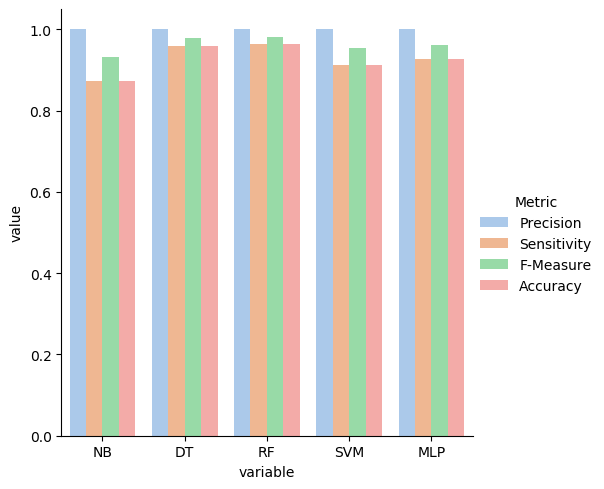
\includegraphics[width=0.49\textwidth]{levenshtein5k_on_phishtank_0401.png}	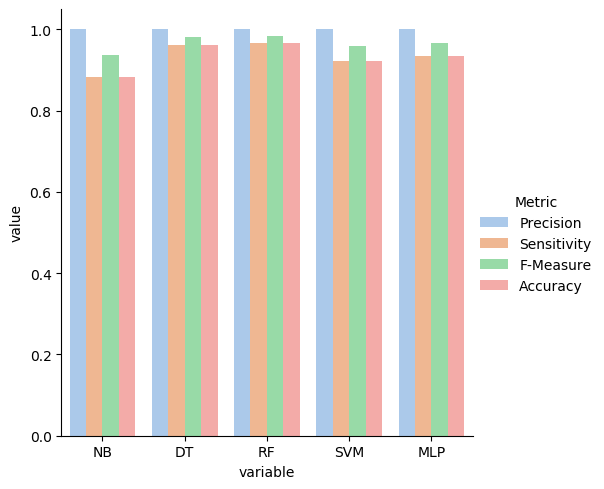
\includegraphics[width=0.49\textwidth]{levenshtein5k_on_phishtank_0405.png}
	\caption{URL length distribution over a dataset of 50,000 records}
	\label{fig:HAMMING_ON_MIXED}
\end{figure}

\begin{figure}[b]
	\centering
	\includegraphics[width=0.49\textwidth]{levenshtein5k_on_mixed.png}
	\caption{URL length distribution over a dataset of 50,000 records}
	\label{fig:HAMMING_ON_MIXED}
\end{figure}

The Hamming distance is designed to calculate the distance between two strings of equal length. Because of this, when computing the Hamming distance between two domains one of them needs to be padded. Because of this the Hamming distance is swapped for the Levenshtein distance. There is no performance loss expected as \cite{SVM_SIMILARITY_INDEX} reports similar results in both similarity indexes. Furthermore, the levenshtein distance will not only be calculated between the malicious domain and benign list of domains, but between the list of benign domains and both malicious subdomain strings separated by periods and the domain. The aim of this addition is to increase model's awareness regarding domains such as "www.bank.secure.brand.com".

One feature that is introduced is the use of sensitive vocabulary.SPEAK ABOUT REF OF SENSITIVE VOCABULARY

SPEAK ABOUT NOT CHOSING HTTP/HTTPS AS FEATURE

The size of the URL and IP presence features are be kept unchanged


1. Dont forget to discuss dataset exploration
2. Speak about not using HTTPS
3. Speak about sensitive words and the selection built
4. Mention that the aim is for this artefact tot be lightweight and show how much plain static URL analysis can achieve
5. Revisit the number of phishing attacks

\section{Performance assessment}


%=========================================================================================================
% Skipped compiling instructions
\iffalse
You should always start with an overview (Heading 2 style) to tell what this chapter is about and finish with a summary (Heading 2 style) to tell what has been covered in this chapter.

The Design and Implementation chapter should explain the design technique chosen and justify why it is appropriate, depending on the development methodology.  Suitable diagram-techniques (e.g. UML, other drawings) should be used where appropriate. For the Implementation part, it should talk about the technical realisation of the concepts and ideas developed earlier. It is used to describe the system at a finer level of technical details, down to the code level. However, do not attempt to describe all the code in the system, and do not include large pieces of code in this section. 

You should highlight the pieces of code which are critical to the system or worth to be noted. For example, the creation and/or implementation of core algorithms that make the system functional or some methods/ways you have used which are non-standard or innovative in the system implementation. You should also mention any unforeseen problems you encountered when implementing the system and how and to what extend you overcame them.

Appropriate testing must also be included in this section
\fi

%!TEX root = ../main.tex
\chapter{Evaluation}
The evaluation chapter measures the achievement of the aim set in the introduction. Also, to better place the artefact in the landscape of existing solutions, the evaluation is presented in direct comparison with GSB and the solutions presented by the literature.

\section{Google Safe Browsing}
The work presented throughout this dissertation aims to challenge and improve the current status quo of browser embedded anti-phishing detection systems. The artefact has successfully almost doubled the classification accuracy while respecting the priorities of such software. By design, it is geared towards delivering a minimal amount of false-positives, at the expense of a slight growth in the number of false negatives. This way, its alerts are trustworthy and do not produce noise. Furthermore, it manages to do so using just the URL of the webpage and does not rely on third-party services for any other information.

Table \ref{tab:ARTEFACT_VS_GSB} shows a comparison between the classification accuracy of both GSB and the artefact. We can observe that the artefact managed to surpass GSB's effectiveness in every instance of the testing process.

Besides classification accuracy, the artefact presents a much simpler structure while causing a disproportionally low number of false-negatives and false-positives. The addition of blacklists, whitelists and other mechanisms is expected to reduce the number of inaccurate predictions further.

\begin{singlespace}
	\begin{center}
		\label{tab:ARTEFACT_VS_GSB}
		\begin{tabular}{  m{16em}  m{12em}  m{7em} } \toprule

			                                    & \textbf{Google Safe Browsing} & \textbf{Artefact} \\ \midrule

			\textbf{Phishtank 01.04.2020}       & 50.76\%                       & 95.61\%           \\

			\textbf{Phishtank 05.04.2020}       & 48.32\%                       & 95.67\%           \\

			\textbf{Phishtank 05.05.2020 (API)} & 44.47\%                       & 94.80\%           \\

			\textbf{Phishtank 06.05.2020 (API)} & 44.33\%                       & 94.78\%           \\

			\textbf{Phishtank 07.05.2020 (API)} & 44.94\%                       & 94.75\%           \\

			\textbf{Phishtank 08.05.2020 (API)} & 45.34\%                       & 94.63\%           \\

			\textbf{Phishtank 09.05.2020 (API)} & 45.33\%                       & 94.64\%           \\

			\textbf{Phishtank 10.05.2020 (API)} & 43.60\%                       & 95.08\%           \\ \bottomrule
		\end{tabular}
		\captionsetup{type=table}\caption{Classification accuracy comparison between GSB and the artefact}
	\end{center}
\end{singlespace}

\section{Literature}
Besides accomplishing the aim of surpassing GSB's performance, the artefact presents competitive results even when compared to what the literature presents. Table \ref{tab:EXISTENT_SOLUTIONS_COMPARISON} shows that when placing the artefact in the comparison of solutions presented by \cite{Adebowale}, its accuracy comes above all others. Moreover, it is trained on a wide range of international phishing URLs, which gives the model language independence.

\begin{center}
	\begin{tabular}{  m{0.5em}  m{6em}  m{13.3em}  m{8.5em}  m{2.3em}  m{4.3em}  } \toprule

		                                & \textbf{Plugin }      & \textbf{Features \& Techniques}      & \textbf{Browser}    & \textbf{Acc}   & \textbf{Type}     \\ \midrule

		\multicolumn{1}{r}{\textbf{1}}  & GoldPhish             & Heuristics \& Features-based         & IE                  & 98             & Free              \\

		\multicolumn{1}{r}{\textbf{2}}  & Cloudmark             & Heuristics                           & IE                  & 94             & Free              \\

		\multicolumn{1}{r}{\textbf{3}}  & SmartScreen           & Blacklist and whitelist              & IE                  & 95.9           & Free              \\

		\multicolumn{1}{r}{\textbf{4}}  & Netcraft              & Blacklist and whitelist              & Chrome, Firefox     & 90             & Free              \\

		\multicolumn{1}{r}{\textbf{5}}  & SpoofGuard            & Heuristics \& Features-based         & IE                  & 91             & Free              \\

		\multicolumn{1}{r}{\textbf{6}}  & Phishdentity          & Google search-by-image API           & IE                  & 97.2           & Research          \\

		\multicolumn{1}{r}{\textbf{7}}  & PhishTackle           & Heuristics \& Features-based         & IE                  & 91.3           & Research          \\

		\multicolumn{1}{r}{\textbf{8}}  & PhishGuard            & Heuristics                           & Firefox             & 94             & Research          \\

		\multicolumn{1}{r}{\textbf{9}}  & PhishIdentifier       & Heuristics                           & Firefox             & 92             & Research          \\

		\multicolumn{1}{r}{\textbf{10}} & PhishTester           & Heuristics \& Features-based         & IE                  & 97.1           & Research          \\

		\multicolumn{1}{r}{\textbf{11}} & CANTINA+              & Heuristics \& Features-based         & IE                  & 98.06          & Research          \\

		\multicolumn{1}{r}{\textbf{12}} & PhishAri              & Features-based                       & Chrome              & 92.52          & Research          \\

		\multicolumn{1}{r}{\textbf{13}} & PhishShield           & Heuristics \& Feature-based          & Chrome              & 96.57          & Research          \\

		\multicolumn{1}{r}{\textbf{14}} & PhishNet              & Blacklist                            & Chrome              & 95             & Research          \\

		\multicolumn{1}{r}{\textbf{15}} & PhishDef              & Heuristics \& Feature-based          & Chrome              & 97             & Research          \\

		\multicolumn{1}{r}{\textbf{16}} & GSB                   & Blacklist                            & Chrome, Firefox     & 93.3           & Free              \\

		\multicolumn{1}{r}{\textbf{17}} & PhishZoo              & Heuristics                           & Chrome              & 96.10          & Research          \\

		\multicolumn{1}{r}{\textbf{18}} & Seclayer              & Heuristics                           & IE, Chrome          & 91             & Free              \\

		\multicolumn{1}{r}{\textbf{19}} & IPDPS                 & Heuristics, Feature and image        & IE, Chrome, Firefox & 98.55          & Research          \\ \midrule

		\multicolumn{1}{r}{\textbf{20}} & \textbf{The artefact} & \textbf{Heuristics \& Feature-based} & \textbf{N/A}        & \textbf{99.29} & \textbf{Research} \\ \bottomrule
	\end{tabular}
	\captionsetup{type=table}\caption{A comparison of existing solutions \citep{Adebowale}}
	\label{tab:EXISTENT_SOLUTIONS_COMPARISON}
\end{center}

\section{Chapter overview}
This chapter assessed classifier's performance and aim accomplishment by comparing the results presented in the previous chapter against both GSB and the relevant solutions proposed by the literature. This comparison shows that the artefact outperforms GSB by a large margin, and manages to rank first when placed between literature solutions.



%!TEX root = ../main.tex
\chapter{Conclusion}
This chapter summarises the work presented throughout this dissertation, progressing through the steps followed to achieve the result. The following subsection lays out the evaluation of the artefact and discusses it's achievents vis-a-vis the set of objectives. The final subsection proposes possible paths of furthering the work presented, expands on the artefact's limitations and possible improvements.

\section{Summary}
The work and presented throguhout this dissertation aimed to challenge and improve the status-quo of browser anti-phishing detection systems. In doing so the objectives have been set around studying the current situation of the most popular browser anti-phishing detection system, surpass it's effectiveness and offer an easy to operate interface with the artefact produced.

The evaluation of Google Safe Browsing has been performed both through a realistic scenario using browser automation and the public Google Safe Browsing API. This analysis has uncovered that feeding the same phishing URLs after a period of time in the detection system results in a lower detection rate in the latter case, thus showing that it's classification influences the lifespan of a phishing webpage. Besides this, the false-negatives rate is consistently low and the process of including new online and valid phishes is slow.

After the evaluation the solution is built and experimented with. The first aim of the solution design is to be lightweight and deliver predictions only when necessary, thus it includes a white list of top one million domains known to be benign. The second aim is the delivery of accurate predictions based only on the URL of the webpage. Besides accuracy, the solution has to be on par with Google Safe Browsing with regards to false positives and false negatives.
Because of the only source of data is the URL, a great amount of research and attention went into building the feature set. Extracting these features and training the first set of models reflects this by delivering substantially better results than the set threshold in both train and test data.

The performance improvement phase outlines the design decision of prioritising a balanced, robust solution instead of a phishing-detection optimised one. This is reflected in the 80\% phishing detection rate on a new test set, while the overall accuracy is 98.91\%. Although it is slightly less than what the literature presents, it is worth considering that the only source of information is the URL, while other solutions use features such as HTML tag analysis, external links analysis and so on.

Finally, the artefact and it's effectiveness despite the reduced data input proves that there is room for improvement in the anti-phishing detection systems available for the public. Furthermore, it's source code is publicly available and perdictions can be delivered by just feeding in the URL.

\section{Objectives review}
The first objective set is to research and develop a mechanism for evaluating the accuracy of the phishing detection system embedded in popular browsers. To address this, a testing tool has been developed that evaluates the accuracy both in a realistic scenario through browser automation and by checking the URLs against Google Safe Browsing's API.

The second objective is to research and corroborate different anti-phishing methods described in the literature into a multi-layered phishing detection design. In doing so, the artefact doesn't only use features described by the literature, but slightly alters some and introduces some new ones. 

The third and last objective is to implement and calibrate a phishing detection system that improves the status quo and can be operated with minimal technical literacy. The artefact produced achives a performance far surpasing what Google safe browsing offers. Furthermore, the artefact surpasses most of the solutions presented by the literature.

\section{Reflection}
Throughout the work carried out to produce the report and artefact presented, the aim and objectives have slightly evolved as the view on the subject matured. This section will expand some of the changes made to the project proposal (REF) offering justifications for the decisions taken.

The proposal starts with presenting an overview of the project. It defines the problem to be addressed and introduces the project idea. While the goal of offering an anti-phishing detection system that requires minimal technical literacy to operate was not altered, some of the features differ from the ones pitched. The artefact to be produced is described as being capable of recognising algorithmically generated domain names, but studying phishing techniques uncovered that these are usually markers of malware command and control servers. The second feature pitched is the inclusion of a blacklist. Although useful as proved by the literature, the machine learning model exceeded the accuracy expectations and the inclusion of phishtank datasets in a blacklist would tamper with the unbiased comparison between it and GSB.

After creating a low resolution image of the artefact's desing, the proposal briefly describes the method of evaluation. Doing the appropriate research proved that the methodology proposed is rudimentary and inacurate. The design of the evaluation has been changed to include metrics used in the performance assessment of models in data science.

\section{Future work}
There are a number of ways to improve the classifier. Future work on the artefact could address either the blindspots, performance improvements. Another area worth considering is User Experience (UX). This can be significantly improved by wrapping the artefact in a browser extension.

An example of a blindspot is the inability to detect man-in-the-middle attacks. A scenario where the legitimate domain name is resolved to an IP address under the control of a threat actor would go under the radar of the artefact. This is solved by implementing a key-value store of domain names and IP addresses. To keep the artefact lightweith this store could be managed by an Random Access Memory (RAM) database (e.g. Memcached, Redis). Although the implementation of such feature is trivial, it is considered out of the scope of objectives set in Chapter 1(REF).

Although the artefact manages to deliver predictions in a timely manner, the time of whitelist checking can be significantly reduced by using low-level compiled programming languages (e.g. C/C++, Rust). 

Furthermore, the perofrmance can be improved by applying the same classification on all the URLs found in the HTML source code of the page to improve surface coverage and lower the number of false-negatives.

Another idea is to focus on the inter-feature correlations and mine rulesets from combined features as shown by \cite{INTELLIGENT_RULE_MINING}.


% FEATURE TWEAKING + HYPERPARAMETER TUNING? Cannot detect when the legit website is highjacked
% 

\clearpage
\vspace*{\fill}
\begin{center}
\begin{minipage}{.6\textwidth}
\centering 
Report word count:

Artefact word count: (equivalent)
\end{minipage}
\end{center}
\vfill
\clearpage


\iffalse
The Conclusions chapter marks the end of the project report and it is a summary which brings together many of the points that you have made in other chapters, especially in the previous chapter. It is usually 2 – 3 pages long with three sections:
\begin{enumerate}
	\item Summary: summarise what you have achieved and restate the main results
	\item Evaluation: evaluate what you have achieved and how well you have met the objectives
	\item Future work: explain any limitations and how things might be improved.]
\end{enumerate}

\noindent
[Word count should be included at the end of the last section. Please look at section 5.2 and 5.3 of the Project Handbook for word count policy.]
\newline
Word count (main body of the report): 
\\
Word count (artefact): 

\fi


\bibliographystyler{packages/buHarvard}
\nociter{*}
\bibliographyr{01_references}

\bibliographystyleb{packages/buHarvard}
\nociteb{*}
\bibliographyb{02_bibliography}


%!TEX root = ../main.tex
\titleformat{\chapter}[hang]
{\normalfont\Huge\bfseries}{\chaptertitlename\ \thechapter\ -\ }{0pt}{\Huge}
\titlespacing*{\chapter}{0pt}{0pt}{20pt}
\begin{appendices}

	%!TEX root = ../main.tex
\chapter{Project proposal}
\label{appendix:project_proposal}

\begin{center}
	\centerline{Department of Computing and Informatics}
	\centerline{2019-2020 Undergraduate Final Year Project Proposal Form}
\end{center}

\textbf{Degree Title:} Forensic Computing and Security

\textbf{Student's Name:} Andrei Butnaru

\textbf{Supervisor's Name:} Alexios Mylonas

\textbf{Project Title/Area:} A machine learning based solution for preventig access to malicious web resources

\tocless\section{Section 1: Project overview}
\begin{mdframed}
	\tocless\subsection{Problem definition - use one sentence to summarise the problem}
	Computer security solutions evolve every day, and this tends to leave behind the use case of the average user who wants to know they’re safe, without having to go through training, maintain software or protection solutions.

	\tocless\subsection{Project description - briefly explain your project:}
	The project’s goal is to serve as a filter against malicious domain names/URLs. The filter will be composed of several subcomponents. These include a blacklist and two machine learning models. The first module predicts maliciousness and the second, whether the domain name is algorithmically generated.

	\tocless\subsection{Project description - briefly explain your project:}
	The project comes as an answer to the main attacks executed across industries today. The way threat actors can circumvent almost any network, or end-point protection solutions are through social engineering. The target of a social engineering attack may be information extraction from a human or pushing the subject to access \end{mdframed} \begin{mdframed} malicious external resources. Given the nature of such attack, there are not many existing solutions other than staff training which is expensive and tedious in some cases.

	\tocless\subsection{Aims and objectives – what are the aims and objectives of your project?}
	The project aims to provide an efficient mechanism for protection against phishing and control of installed malware for non-technical and technical individuals alike. The project goals are to (1) prevent the user from accessing external malicious resources and (2) in the case of infection, prevent unacknowledged connections to external machines or resources (e.g. command and control servers).
	On the way of achieving the aim, the following objectives are used as a way of quantifying achievement:
	\begin{itemize}
		\item The project features an updated blacklist of phishing and malicious domains names/URLs.
		\item If the domain name/URL passes the blacklist test, the product of the project is able to determine if it is malicious using a trained machine learning model.
		\item The project is able to categorise a domain name as algorithmically generated or not.\newline
	\end{itemize}
\end{mdframed}


\tocless\section{Section2: Artefact}
\begin{mdframed}
	\tocless\subsection{What is the artefact that you intend to produce?}
	The artefact produced will be able to take a domain name/URL as an input, and output a prediction on the maliciousness of it (under the form of a percentage or malicious/non-malicious). It will feature blacklists and two machine learning models. The first model will study the similarities between known malicious domain name/URL, and the second will study the format of algorithmically generated domain names and will categorise the input domain name accordingly.\end{mdframed}

\begin{mdframed}
	\tocless\subsection{How is your artefact actionable (i.e., routes to exploitation in the technology domain)?}
	The artefact is expected to be used as a browser extension, which will supervise the domains and URLs accessed by the user, or as a filter mechanism deployed on central resources such as routers or domain name servers.
\end{mdframed}

\tocless\section{Evaluation}
\begin{mdframed}
	\tocless\subsection{How are you going to evaluate your work?}
	The evaluation will be done by first deploying the artefact on a machine after which:

	• The blacklist will be evaluated by feeding them back to the artefact
	• The test data (malicious URLs) will be fed into the first trained model and see the rate of success and false positives
	• The test data (generated and benign domain names) will be fed into the second trained model and see the rate of success and false positives

	\tocless\subsection{Why is this project honours worthy?}
	In my opinion, this project is honours worthy because it is built on everything I learned throughout my course, plus further research into other domains such as automated testing and machine learning. Another reason is that all this effort goes into a piece of software that is meant to be used by anyone, independent of their understanding of computer security, for a safer internet.


	\tocless\subsection{How does this project relate to your degree title outcomes?}
	The project I’ve chosen fits perfectly in my course title. It requires the knowledge I acquired from almost all the subjects I’ve studied. It will be heavily dependent on what I learned throughout Ethical Hacking and Countermeasures, Digital Forensics, Computers and Networks and Programming. Moreover, it pushes me to develop skills in data science to accomplish the aim.
\end{mdframed}
\begin{mdframed}
	\tocless\subsection{How does your project meet the BCS Undergraduate Project Requirements?}
	I would say the project is a perfect fit for what the BCS presents as their purpose: “To promote and advance the education and practice of computing for the benefit of the public”. I am working towards delivering the best solution I am capable of, with the end goal of serving public safety.


	\tocless\subsection{What are the risks in this project and how are you going to manage them?}
	The biggest risk of the project would be to end up with an implementation that has an undesirable rate of success. By the rate of success, it is to be understood a high rate of false positives, a high rate of false negatives or both. I am planning on managing this risk by tweaking the detection algorithm and calibrate it in a way that improves the success rate, and I have allocated 30 days for this process.
\end{mdframed}

\tocless\section{Ethics}
\begin{mdframed}
	\tocless\subsection{Have you submitted online ethics checklist to your supervisor? \textbf{Yes}/No}
	\tocless\subsection{Has the checklist been approved by your supervisor? \textbf{Yes}/No}
\end{mdframed}

\tocless\section{Proposed plan}
See Appendice \ref{appendix:gantt_chart}
	%!TEX root = ../main.tex
\chapter{GANT Chart}
	%!TEX root = ../main.tex

\chapter{Model configurations}
\label{appendix:model_configurations}

\section{Naive bayes}
\begin{verbatim}
    "name": "Naive Bayes", "filename": "naive_bayes", "model": GaussianNB()
\end{verbatim}

\section{Decision tree}
\begin{verbatim}
        "name": "Decision Tree",
        "filename": "decision_tree",
        "model": DecisionTreeClassifier(random_state=1)

\end{verbatim}

\section{Random forest}
\begin{verbatim}
        "name": "Random Forest",
        "filename": "random_forest",
        "model": GridSearchCV(
            RandomForestClassifier(random_state=1),
            [
                {
                    "n_estimators": [150, 295, 350],
                    "max_features": ["auto"],
                    "min_samples_split": [8, 12],
                    "max_depth": [15, 18, 21],
                }
            ],
            cv=5,
        )
\end{verbatim}

\section{Support vector machine}
\begin{verbatim}
        "name": "Support Vector Machine",
        "filename": "support_vector",
        "model": GridSearchCV(
            SVC(kernel="rbf", random_state=1),
            [{"C": [1, 10, 100, 1000],}],
            cv=5,
        )
\end{verbatim}

\section{Multilayered perceptron}
\begin{verbatim}
        "name": "Neural Network",
        "filename": "ml_perceptron",
        "model": GridSearchCV(
            MLPClassifier(max_iter=2500),
            [
                {
                    "hidden_layer_sizes": [
                        (25, 50, 25),
                        (50, 50, 50),
                        (50, 100, 50),
                        (100,),
                    ],
                    "activation": ["tanh", "relu"],
                    "solver": ["sgd", "adam"],
                    "alpha": [0.0001, 0.05],
                    "learning_rate": ["constant", "adaptive"],
                }
            ],
            cv=5,
        )
\end{verbatim}
	%!TEX root = ../main.tex
\chapter{Artefact repository}

\tocless\section{Cloning}
The entire source code of the report and artefact are uploaded to GitHub. To clone the source use the command:
\begin{verbatim}
    git clone git@github.com:abutnaru/dissertation.git
\end{verbatim}

{\parindent0pt Alternatively, the project can be viewed and downloaded by accessing: }

\begin{verbatim}
    https://github.com/abutnaru/dissertation
\end{verbatim}
	%!TEX root = ../main.tex
\chapter{Iterim review}
\textbf{Student: Andrei Butnaru} \textbf{Supervisor: Alexios Mylonas}


\tocless\section{Define the problem}

\begin{mdframed}
    Has the problem been defined, has the artefact been identified and have objectives been set?
    \textbf{Yes}
\end{mdframed}

\tocless\section{Review of Other Work}
\begin{mdframed}
    Is there evidence of appropriate research?
    \textbf{Yes}
\end{mdframed}

\tocless\section{Analysis, Design \& Implementation of Artefact}
\begin{mdframed}
    Is there evidence of appropriate analysis of the problem and development of a solution?
    \textbf{Yes}
\end{mdframed}

\tocless\section{Dissertation}
\begin{mdframed}
    Have sections of the dissertation been written and has the Supervisor seen these?
    \textbf{Yes}
\end{mdframed}

\tocless\section{Planning \& Progress}
\begin{mdframed}
    Is there an acceptable plan for this project and is it being followed?
    \textbf{To some extent}
\end{mdframed}

\textbf{Comments:} The plan has been adjusted, some delays due to the lockout.

    \textbf{Overall Assessment} Satisfactory

\clearpage
\begin{mdframed}

    \textbf{Date:} March 27

    {\parindent0pt \textbf{Signed:} }

    Supervisor: ....Alexios....

    Student: ....Andrei....

\end{mdframed}


• Supervisor to retain the signed form and supply the student with a copy if required.

• Supervisor to upload the form on Brightspace and grade the student as Satisfactory, Requires Major Improvement, Requires Minor Improvement or Unsatisfactory.

• Supervisor to notify the Project Coordinator if the student is at risk of failing the project or not engaging.
	%!TEX root = ../main.tex
\chapter{Train dataset analysis}
\begin{singlespace}
	\begin{table}[h!]
		\begin{center}
			\begin{tabular}{ m{7.9em} m{3.8em} m{3.4em} m{3.3em} m{7em} m{7em}} \toprule
				\textbf{Feature}                                       & \textbf{Label} & \textbf{Average} & \textbf{Median} & \textbf{90th percentile} & \textbf{99th percentile} \\ \midrule  \addlinespace

				\multirow{2}{*}{\textbf{URL length}}                   & Benign         & 57               & 52              & 90                       & 141                      \\ & Phishing & 77 &  58 & 143 & 321     \\  \addlinespace \addlinespace

				\multirow{2}{*}{\textbf{Protocol}}                     & Benign         & 0                & 0               & 0                        & 0                        \\ & Phishing & 0.77 &  1 & 1 & 1     \\  \addlinespace  \addlinespace

				\multirow{2}{*}{\textbf{\makecell[l]{Numerical                                                                                                                     \\ characters}}}    & Benign         & 0.06             & 0               & 0                        & 3                        \\ & Phishing &0.79 &  0&2 & 12     \\  \addlinespace  \addlinespace

				\multirow{2}{*}{\textbf{\makecell[l]{Symbols  count}}} & Benign         & 0                & 0               & 0                        & 0                        \\ & Phishing &0.05 &  0&0 & 1     \\  \addlinespace  \addlinespace

				\multirow{2}{*}{\textbf{\makecell[l]{Other network                                                                                                                 \\ location}}}        & Benign         & 0.01             & 0               & 0                        & 1                        \\ & Phishing &0.17 &  0&1 & 1     \\  \addlinespace  \addlinespace

				\multirow{2}{*}{\textbf{\makecell[l]{Hyphen                                                                                                                        \\ count}}}     & Benign         & 0.06             & 0               & 0                        & 1                        \\ & Phishing &0.39 &  0&1 & 4     \\  \addlinespace  \addlinespace

				\multirow{2}{*}{\textbf{\makecell[l]{Subdomain                                                                                                                     \\ components}}}    & Benign         & 0.06             & 0               & 0                        & 1                        \\ & Phishing &0.05 &  0&0 & 1     \\  \addlinespace  \addlinespace

				\multirow{2}{*}{\textbf{\makecell[l]{Sensitive                                                                                                                     \\ subdomain}}}       & Benign         & 0                & 0               & 0                        & 0                        \\ & Phishing &0.03 &  0&0 & 1     \\  \addlinespace  \addlinespace

				\multirow{2}{*}{\textbf{\makecell[l]{Sensitive                                                                                                                     \\ domain}}}       & Benign         & 0                & 0               & 0                        & 0                        \\ & Phishing & 0.03 &  0&0 & 1     \\  \addlinespace  \addlinespace

				\multirow{2}{*}{\textbf{\makecell[l]{Sensitive                                                                                                                     \\ path}}}      & Benign         & 0                & 0               & 0                        & 0                        \\ & Phishing &0.22 &  0&1 & 1     \\  \addlinespace  \addlinespace
				\multirow{2}{*}{\textbf{\makecell[l]{Network location                                                                                                              \\ in path}}} & Benign         & 0                & 0               & 0                        & 0                        \\ & Phishing &0.01 &  0&0 & 1     \\  \addlinespace  \addlinespace

				\multirow{2}{*}{\textbf{\makecell[l]{Domain                                                                                                                        \\ distance}}}       & Benign         & 0.21             & 0               & 1                        & 1                        \\ & Phishing &9.48 &  0&1 &1     \\  \addlinespace  \addlinespace

				\multirow{2}{*}{\textbf{\makecell[l]{Subdomain                                                                                                                     \\ distance}}}    & Benign         & 0                & 0               & 0                        & 0                        \\ & Phishing &0.86 &  1&1 & 1     \\\bottomrule
			\end{tabular}
			\captionsetup{type=table}\caption{ Optimised random forest results on the 380,000 mixed records dataset}
			\label{tab:FINAL_MODEL}
		\end{center}
	\end{table}
\end{singlespace}


\end{appendices}

\end{document}